% !TEX ROOT=./main.tex



\section{Numerical Experiments}
\label{sec:exp}

In this section, we empirically examine the linear speedup convergence of FedAvg and Nesterov accelerated FedAvg in various settings, including strongly convex function, convex smooth function, and overparameterized objectives, as analyzed in previous sections.

\textbf{Setup.} Following the experimental setting in~\cite{stich2018local}, we
conduct experiments on both synthetic datasets and real-world dataset
w8a~\cite{platt1998fast} $(d=300, n=49749)$. We consider the distributed
objectives $F(\vw) = \sum_{k=1}^N p_kF_k(\vw)$, and the objective function on the
$k$-th local device includes three cases: 1) \textbf{Strongly convex
objective}: the regularized binary logistic regression problem, $F_k(\vw) =
\frac{1}{N_k} \sum_{i=1}^{N_k} \log( 1+ \exp(-y_i^k \vw^T\vx_i^k) + \frac{\lambda}{2}
\|\vw\|^2$. The regularization parameter is set to $\lambda = 1/n \approx
2e-5$. 2) \textbf{Convex smooth objective}: the binary logistic regression
problem without regularization. 3) \textbf{Overparameterized setting}:
the linear regression problem without adding noise to the label, $F_k(\vw) =
\frac{1}{N_k} \sum_{i=1}^{N_k} (\vw^T\vx_i^k + b  - y_i^k)^2$.  
% In the first
% two cases, we use the w8a dataset to conduct empirical evaluation. 
% In the overparameterized setting, we use features from w8a dataset and 
% generate a ground truth $w$ to label each instance, which satisfies the
% overparameterized setting. 

% ~\ref{th:strongcvxsmth}~\ref{th:cvxsmoth}~\ref{th:fedmasslr}
\textbf{Linear speedup of FedAvg and Nesterov accelerated FedAvg.} To verify the linear speedup convergence as shown in Theorems~\ref{thm:SGD_scvx}~\ref{thm:SGD_cvx}~\ref{thm:nesterov_scvx}~\ref{thm:Nesterov_cvx}, we evaluate the number of iterations needed to reach
$\epsilon$-accuracy in three objectives. We initialize all runs with $\vw_0 = \textbf{0}_d$ and measure the number of iterations to reach the target accuracy $\epsilon$. For each configuration $(E, K)$, we extensively search the learning rate from $\min(\eta_0, \frac{nc}{1 + t})$, where
$\eta_0 \in \{0.1, 0.12, 1, 32 \}$ according to different problems and $c$ can
take the values $c = 2^i \ \forall i \in \ZZ$. As the results shown in Figure~\ref{fig:speedup},
the number of iterations decreases as the number of (active) workers increasing, which is consistent for FedAvg and Nesterov accelerated FedAvg across all scenarios.
For additional experiments on the impact of $E$, detailed experimental setup, and hyperparameter setting, please refer to the Appendix Section~\ref{sec:expsupp}.

% \textbf{Partial participations.} We verify the linear speedup in the
% partial participation settings, where we set $50\%$ of devices
% are active. As the results are shown in Figure~\ref{fig:speedup} (2nd row), the 
% FedAve enjoys linear speedup in various settings even with partial
% device participation.

% \textbf{Nesterov accelerated FedAvg.} In the third row of Figure~\ref{fig:speedup}, 
% we report the last iteration to converge to $\epsilon$-accuracy of Nesterov accelerated FedAvg. The empirical observations align with Theorem~\ref{thm:nesterov_scvx}~\ref{thm:Nesterov_cvx} that the accelerated version of FedAvg can also achieve the linear speedup
% w.r.t the number of workers.

% \textbf{The impact of $E$.} We further examine how does the number of local steps ($E$) 
% affect convergence. As shown in Figure~\ref{fig:e} in appendix section~\ref{sec:expsupp}, the number of iterations increases as $E$ increase, which slow down the convergence in
% terms of gradient computation. However, it can save communication costs as
% the number of rounds decreased when the $E$ increases. This showcase that
% we need a proper choice of $E$ to trade-off the communication cost and
% convergence speed. 

\begin{figure}[h!]
\centering
{\small
\begin{tabular}{ccc}
\hspace{-2em}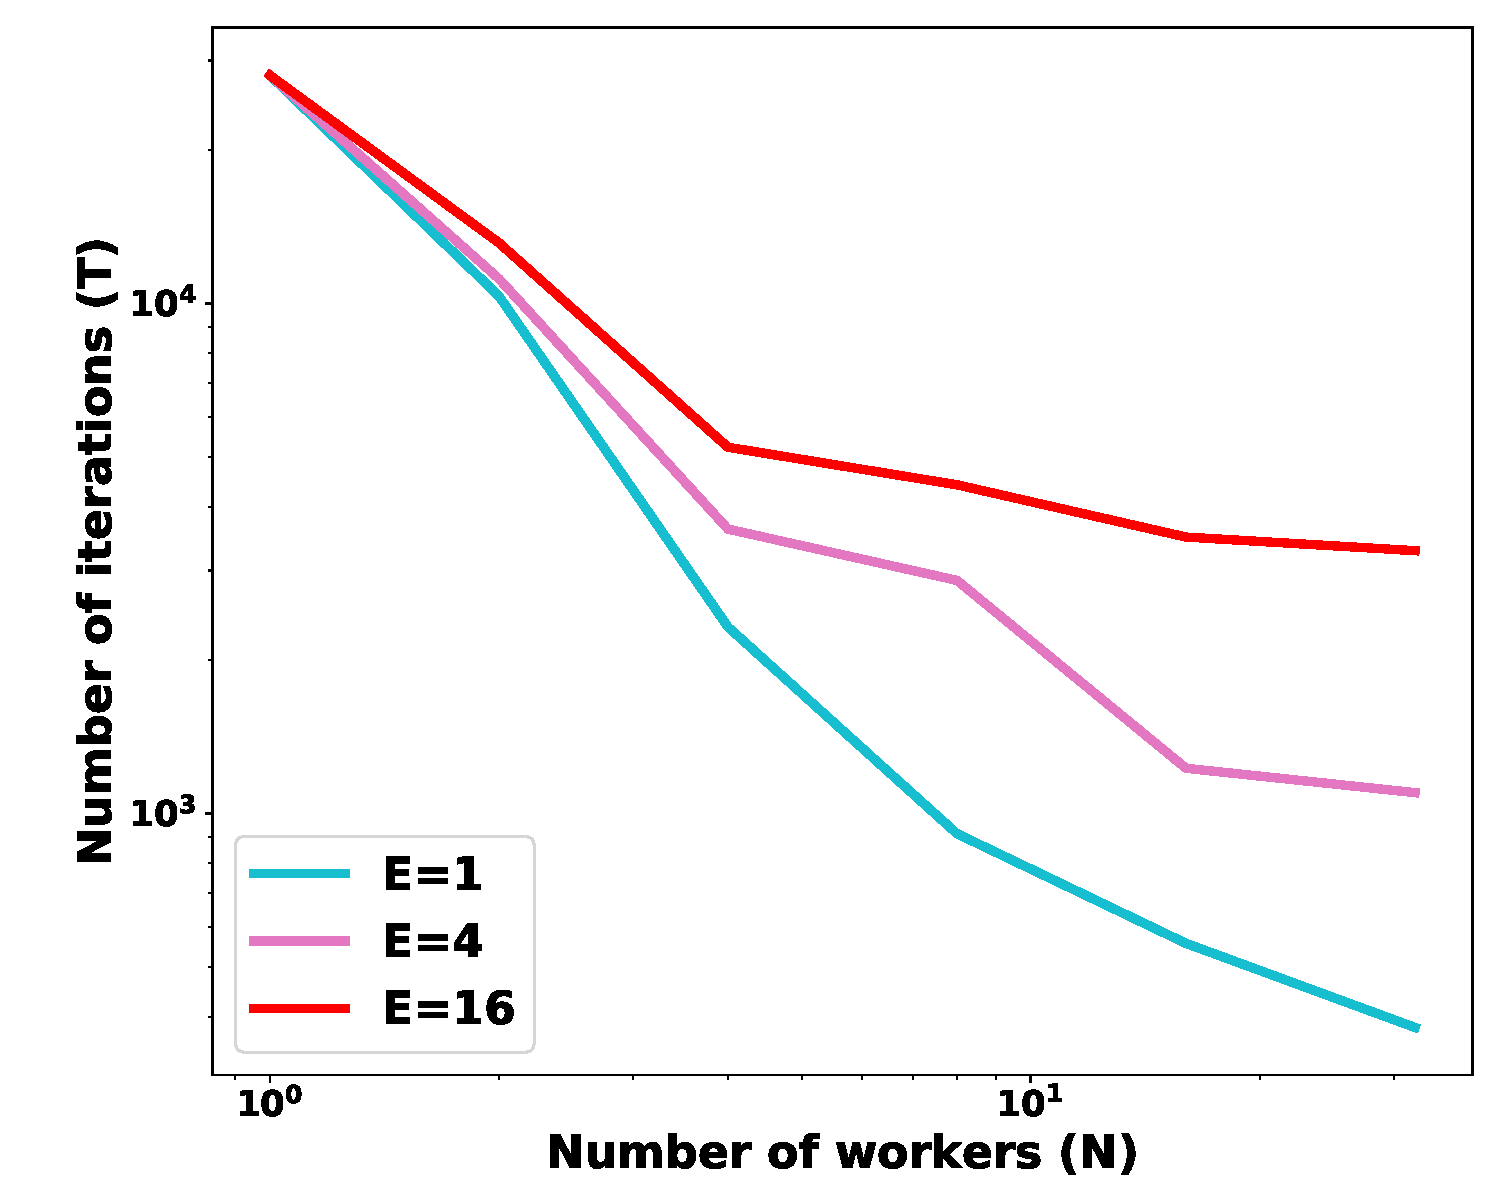
\includegraphics[width=0.33\textwidth]{fig/paper-stronglycvxsmthspeedupNodesT-min-w8a-epsilon0131-reg1e-05.pdf} &
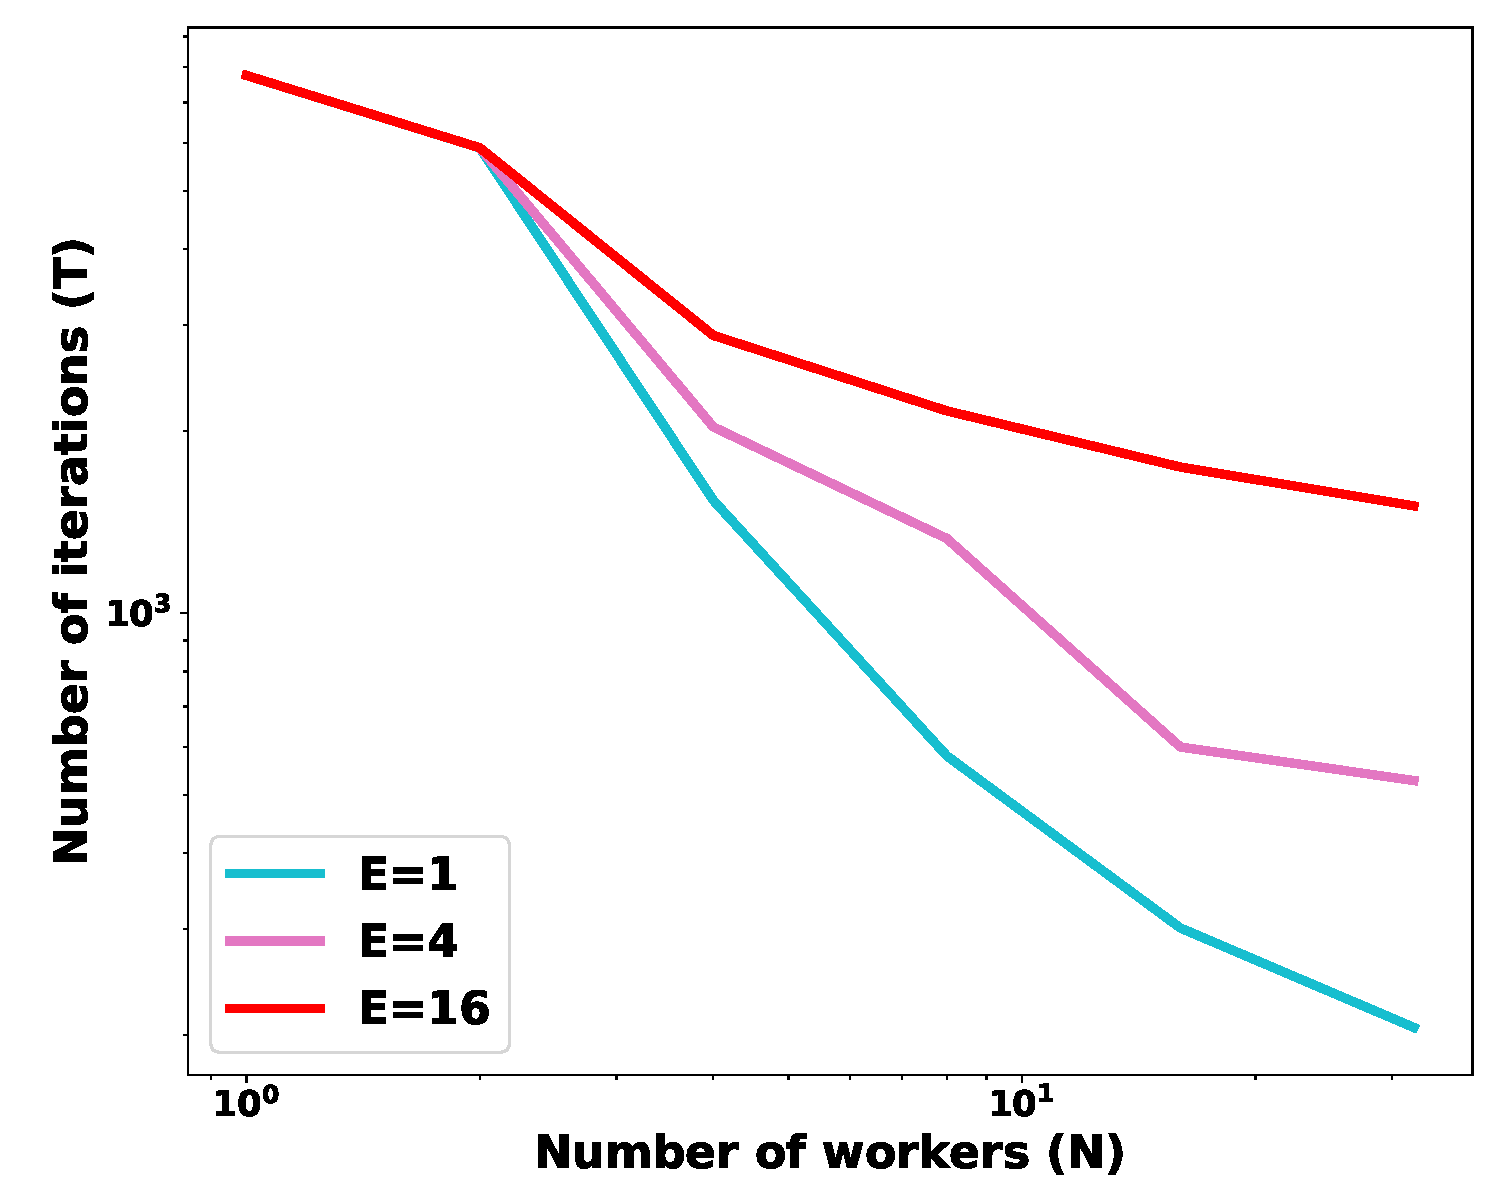
\includegraphics[width=0.33\textwidth]{fig/paper-cvxsmoothspeedupNodesT-min-w8a-epsilon0134-reg0.pdf} &
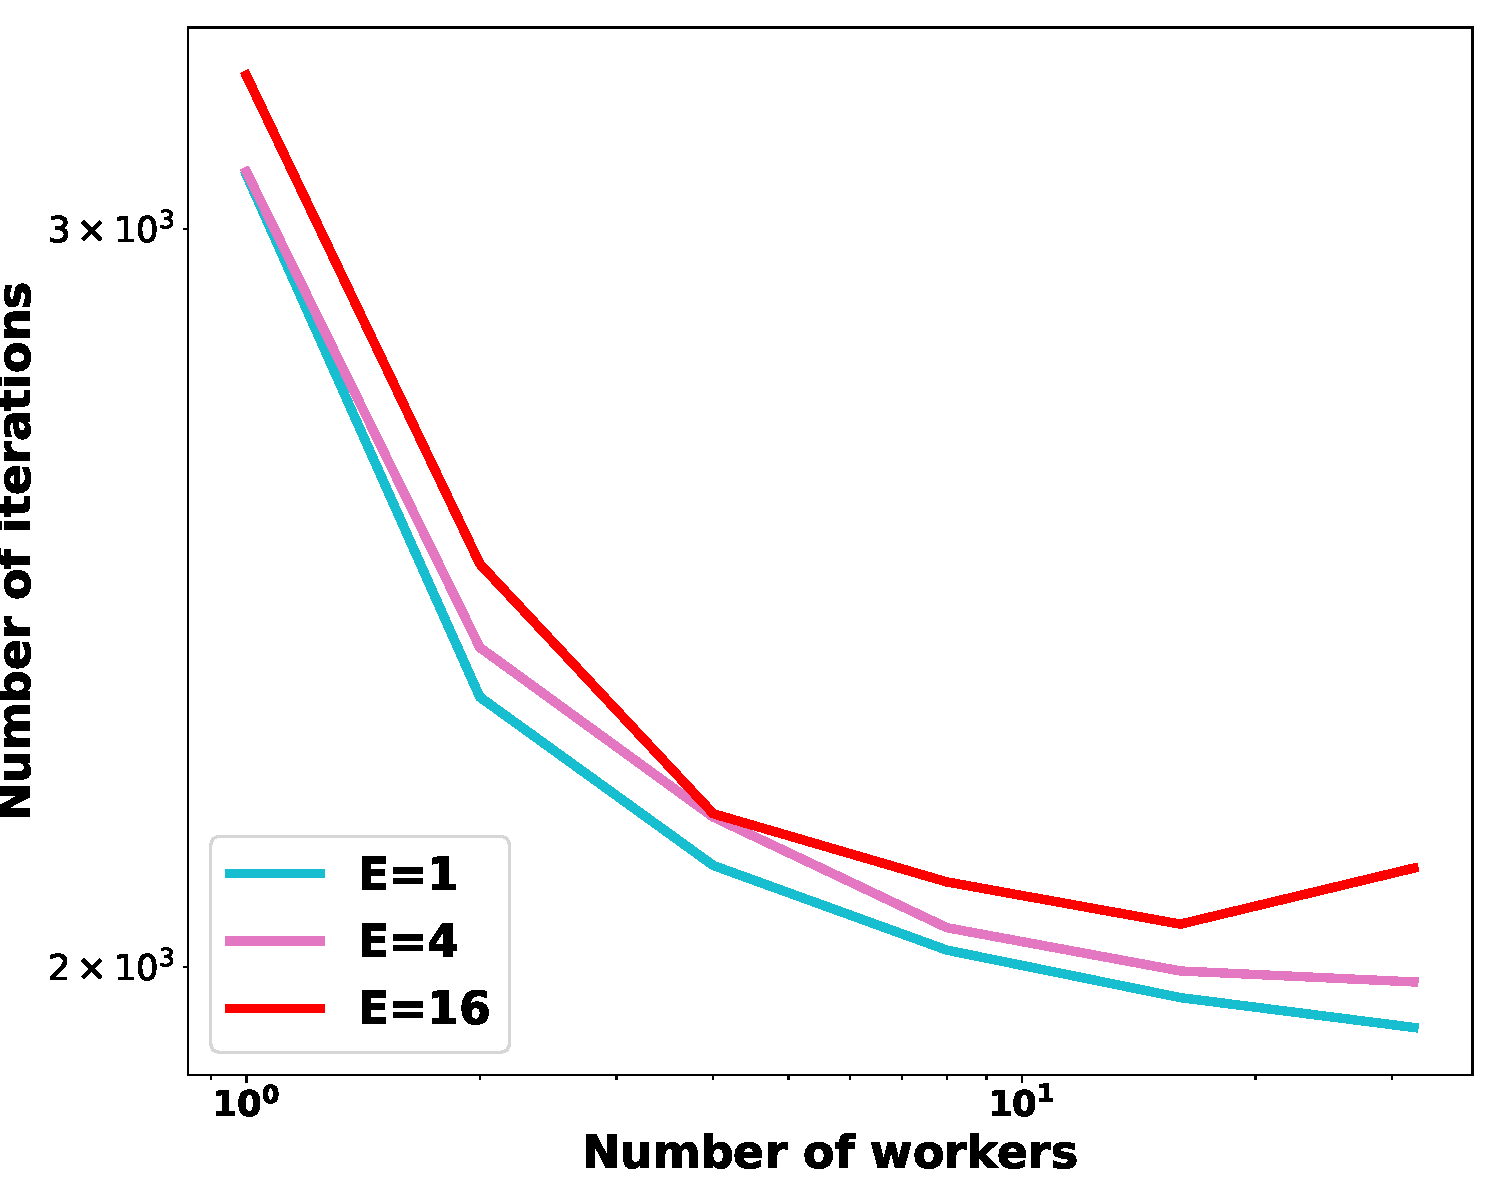
\includegraphics[width=0.33\textwidth]{fig/paper-linregressionspeedupNodesT-min-linearregressionw8a-epsilon002-reg0.pdf}\\
\hspace{-2em}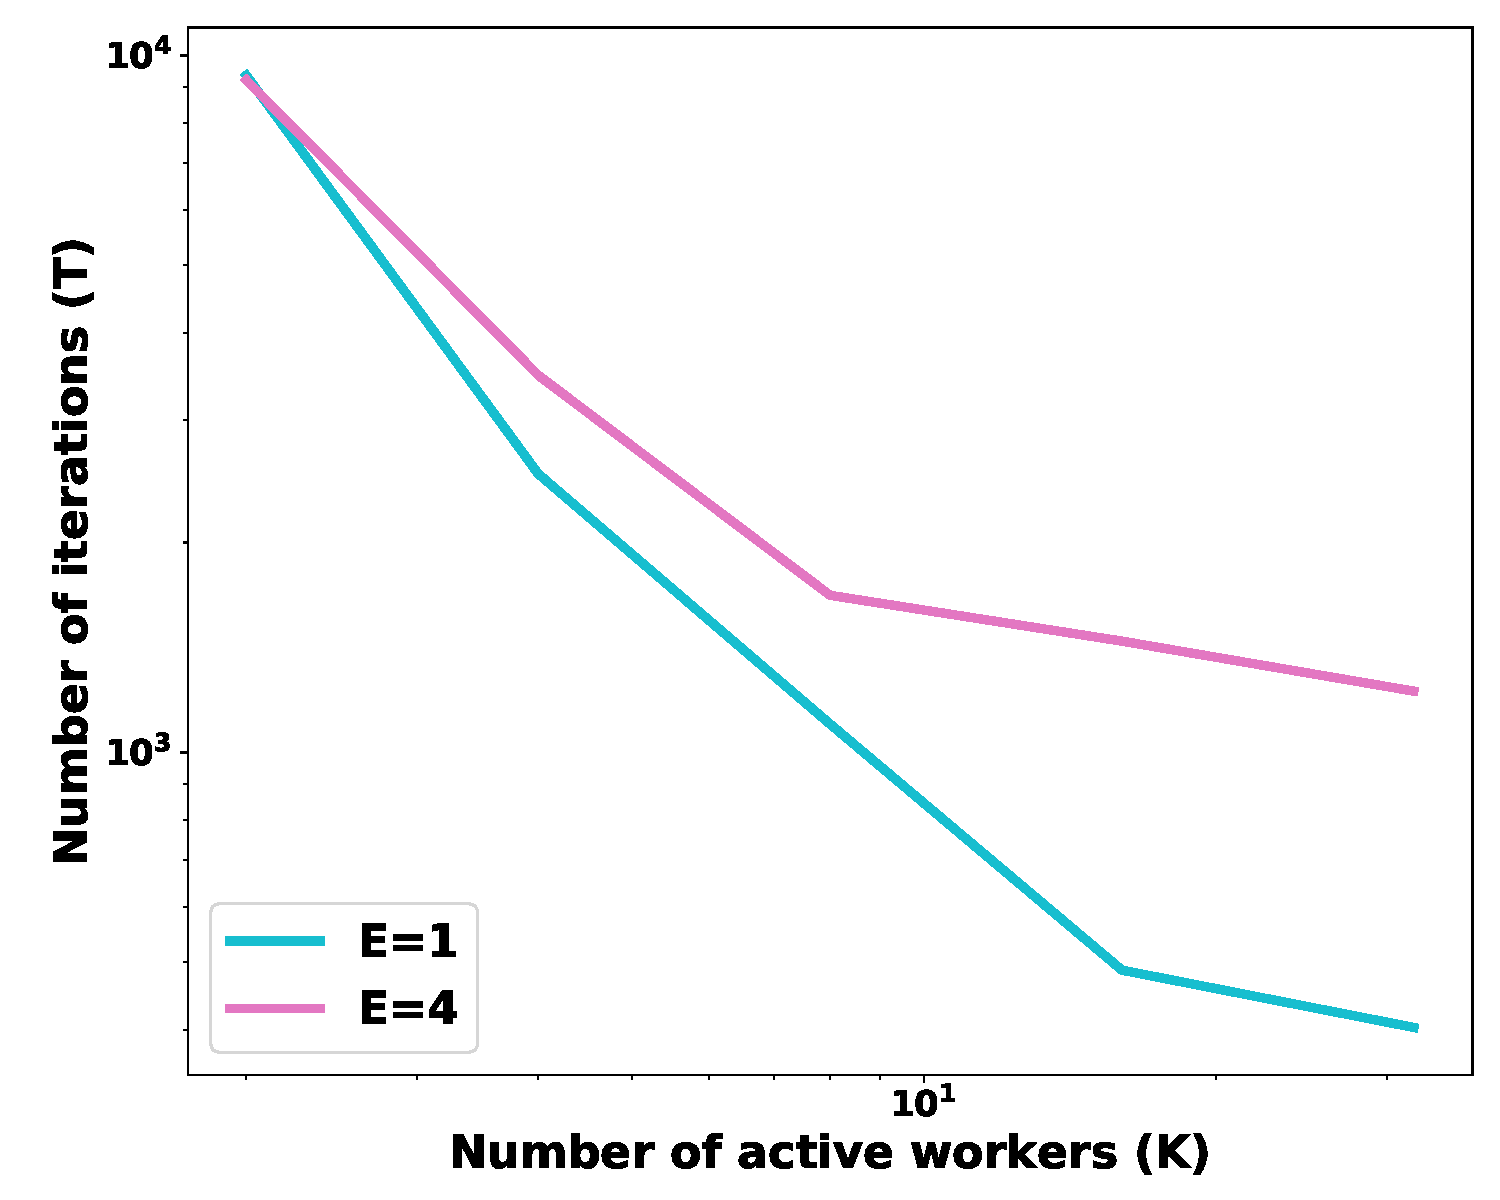
\includegraphics[width=0.33\textwidth]{fig/paper-partialstronglycvxsmthspeedupNodesT-min-w8a-epsilon0131-reg1e-05.pdf} &
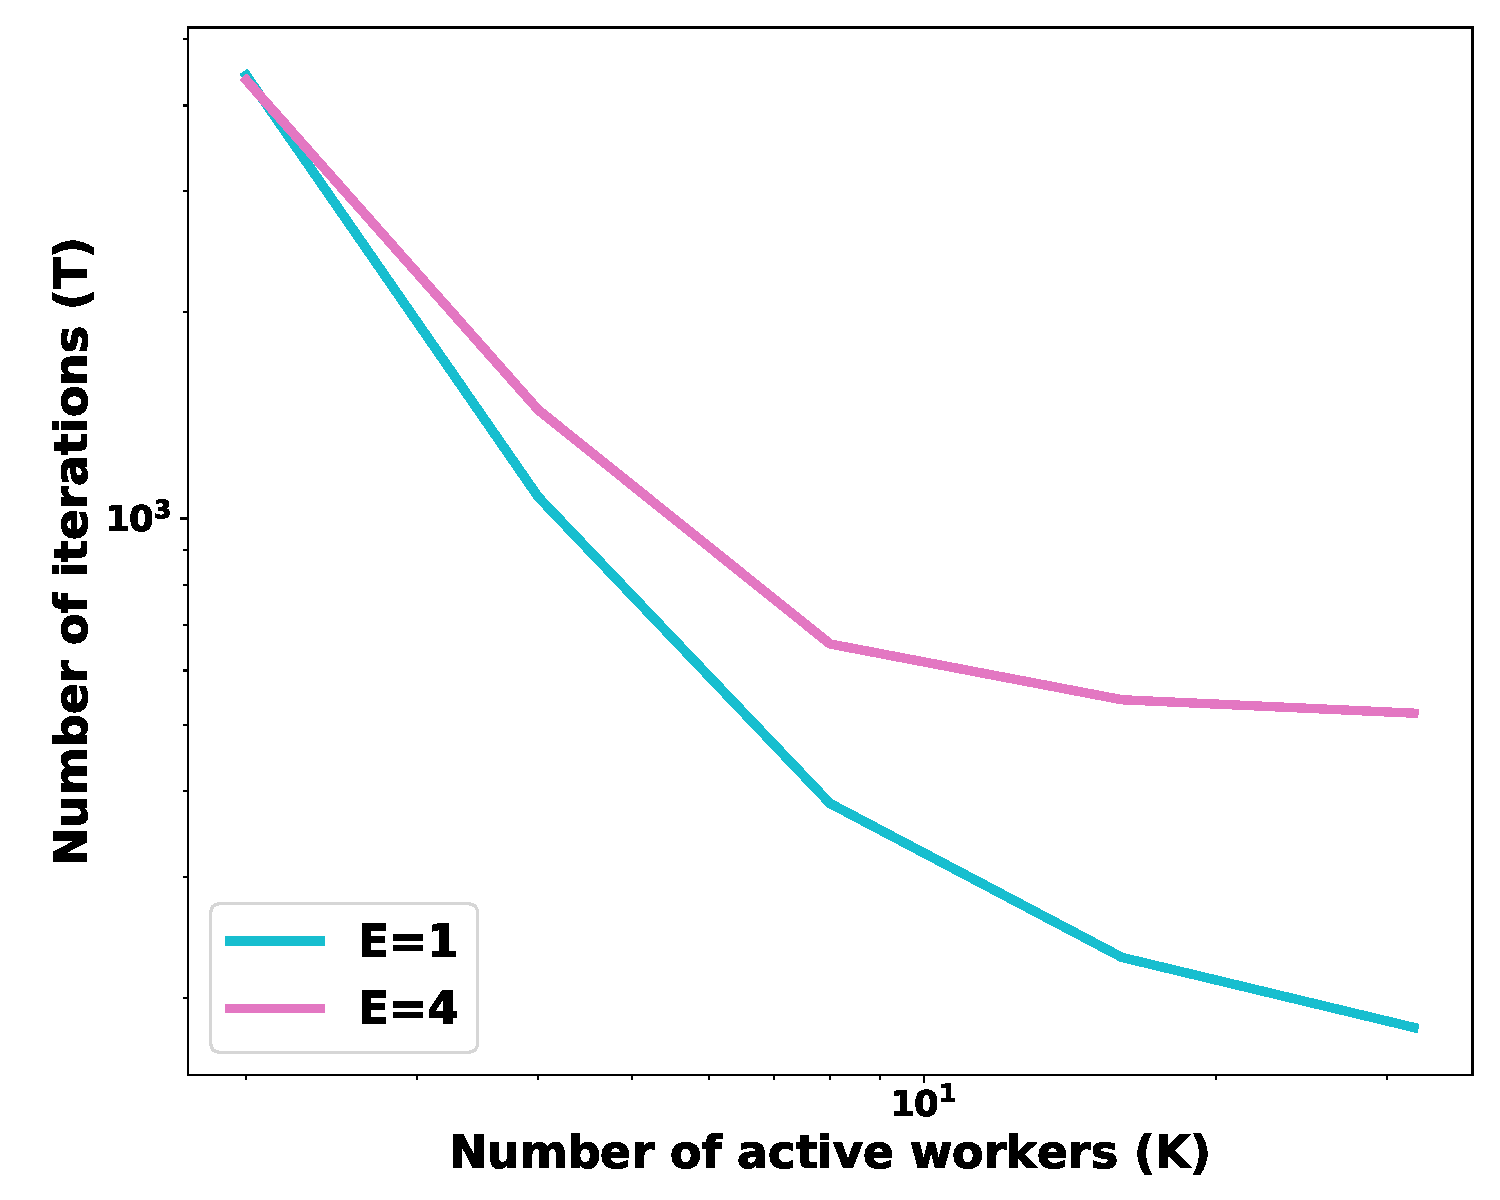
\includegraphics[width=0.33\textwidth]{fig/paper-partialcvxsmoothspeedupNodesT-min-w8a-epsilon0134-reg0.pdf} &
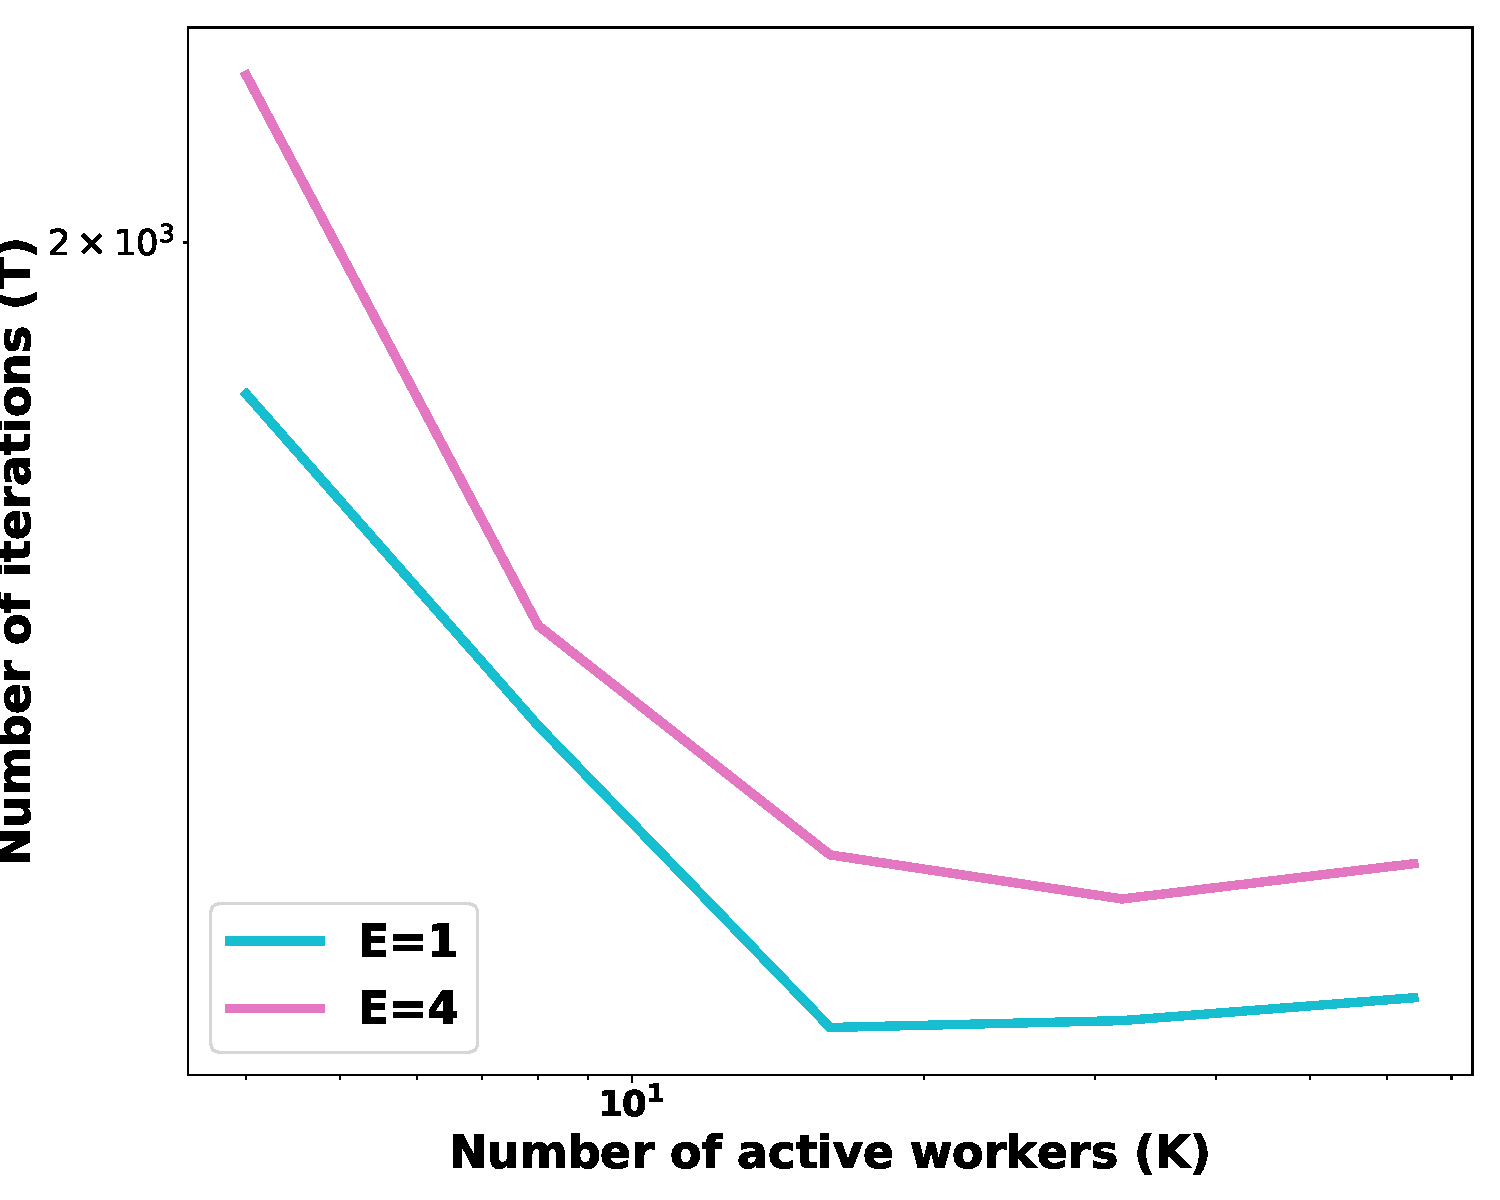
\includegraphics[width=0.33\textwidth]{fig/paper-partiallinregressionspeedupNodesT-min-linearregressionw8a-epsilon002-reg0.pdf}\\
\hspace{-2em}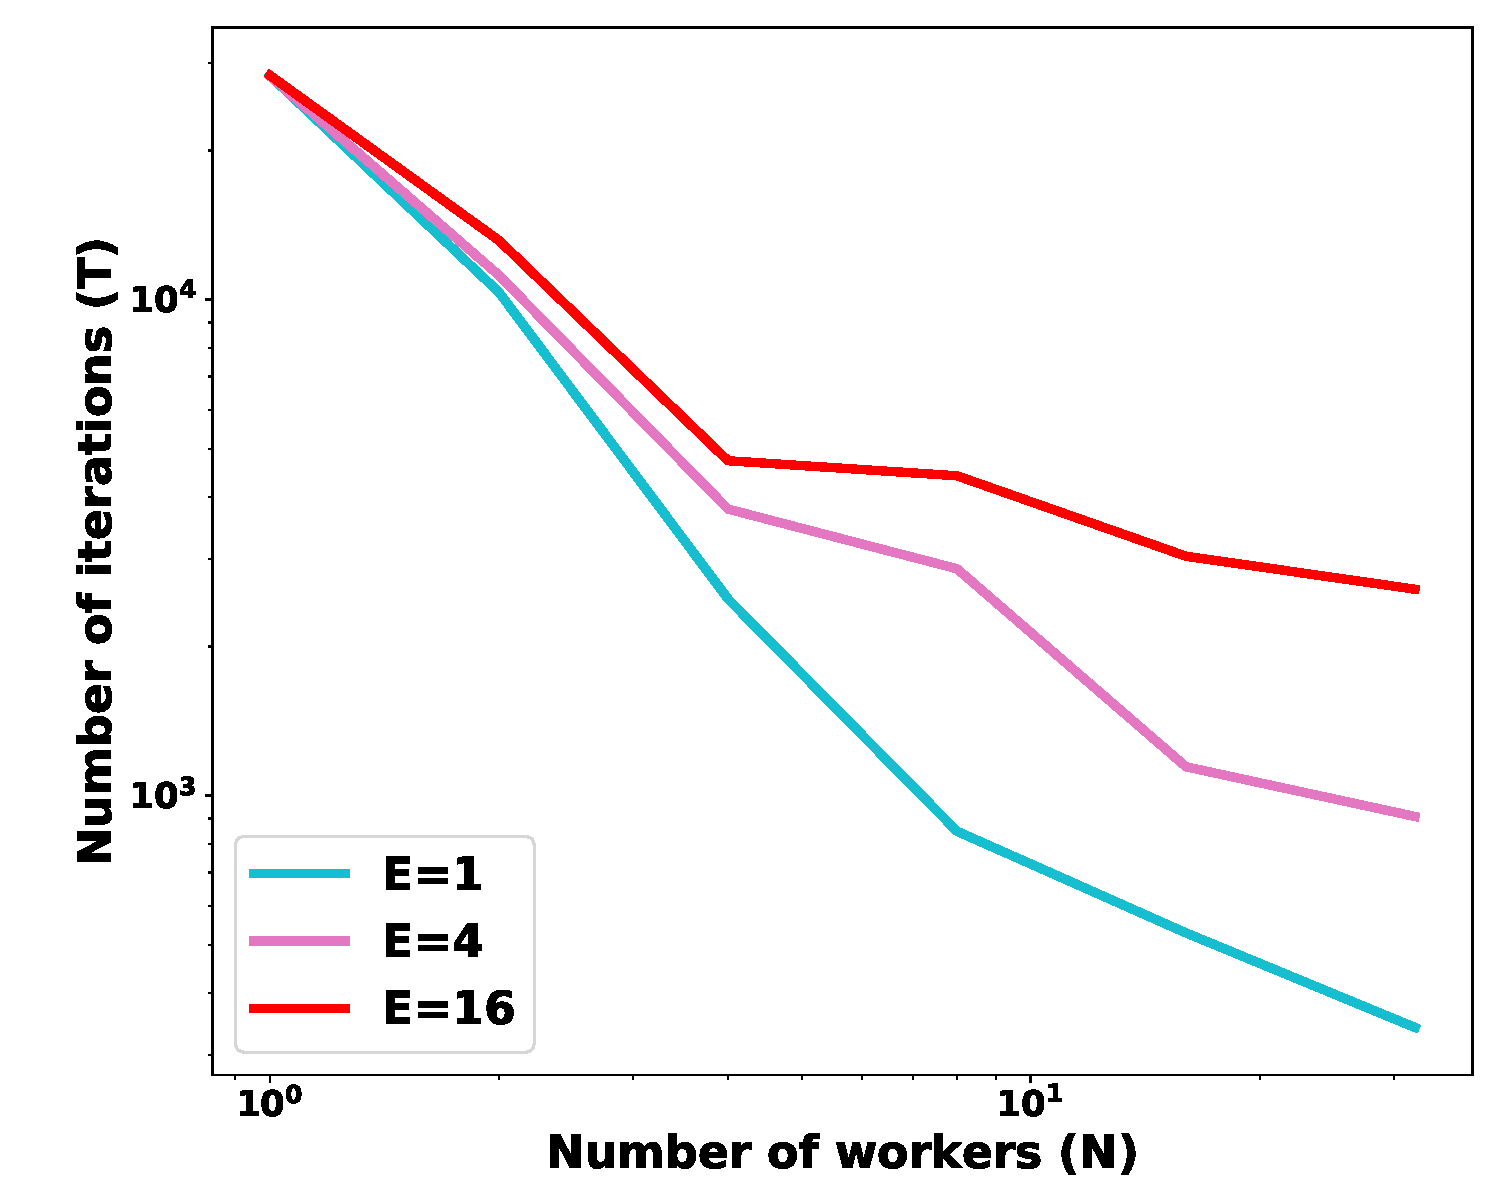
\includegraphics[width=0.33\textwidth]{fig/paper-nesterovspeedupNodesT-min-w8a-epsilon0131-reg1e-05.pdf} & 
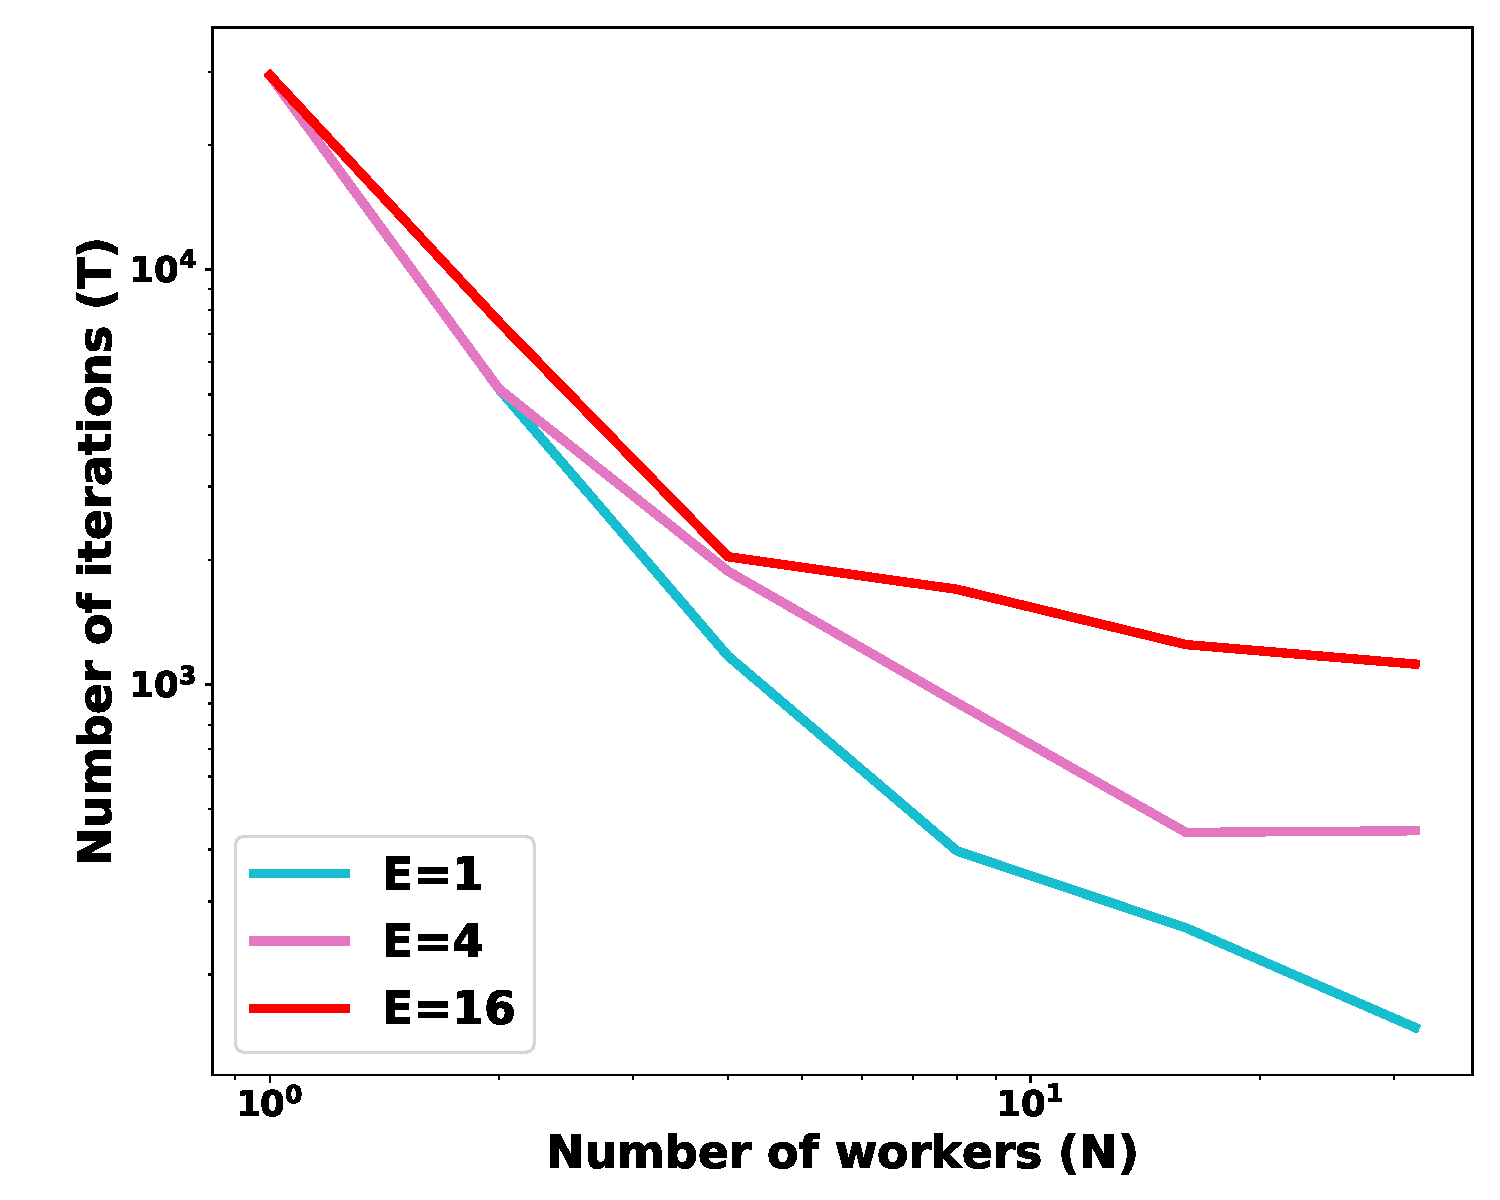
\includegraphics[width=0.33\textwidth]{fig/paper-nesterovspeedupNodesT-min-w8a-epsilon0134-reg0.pdf}
& 
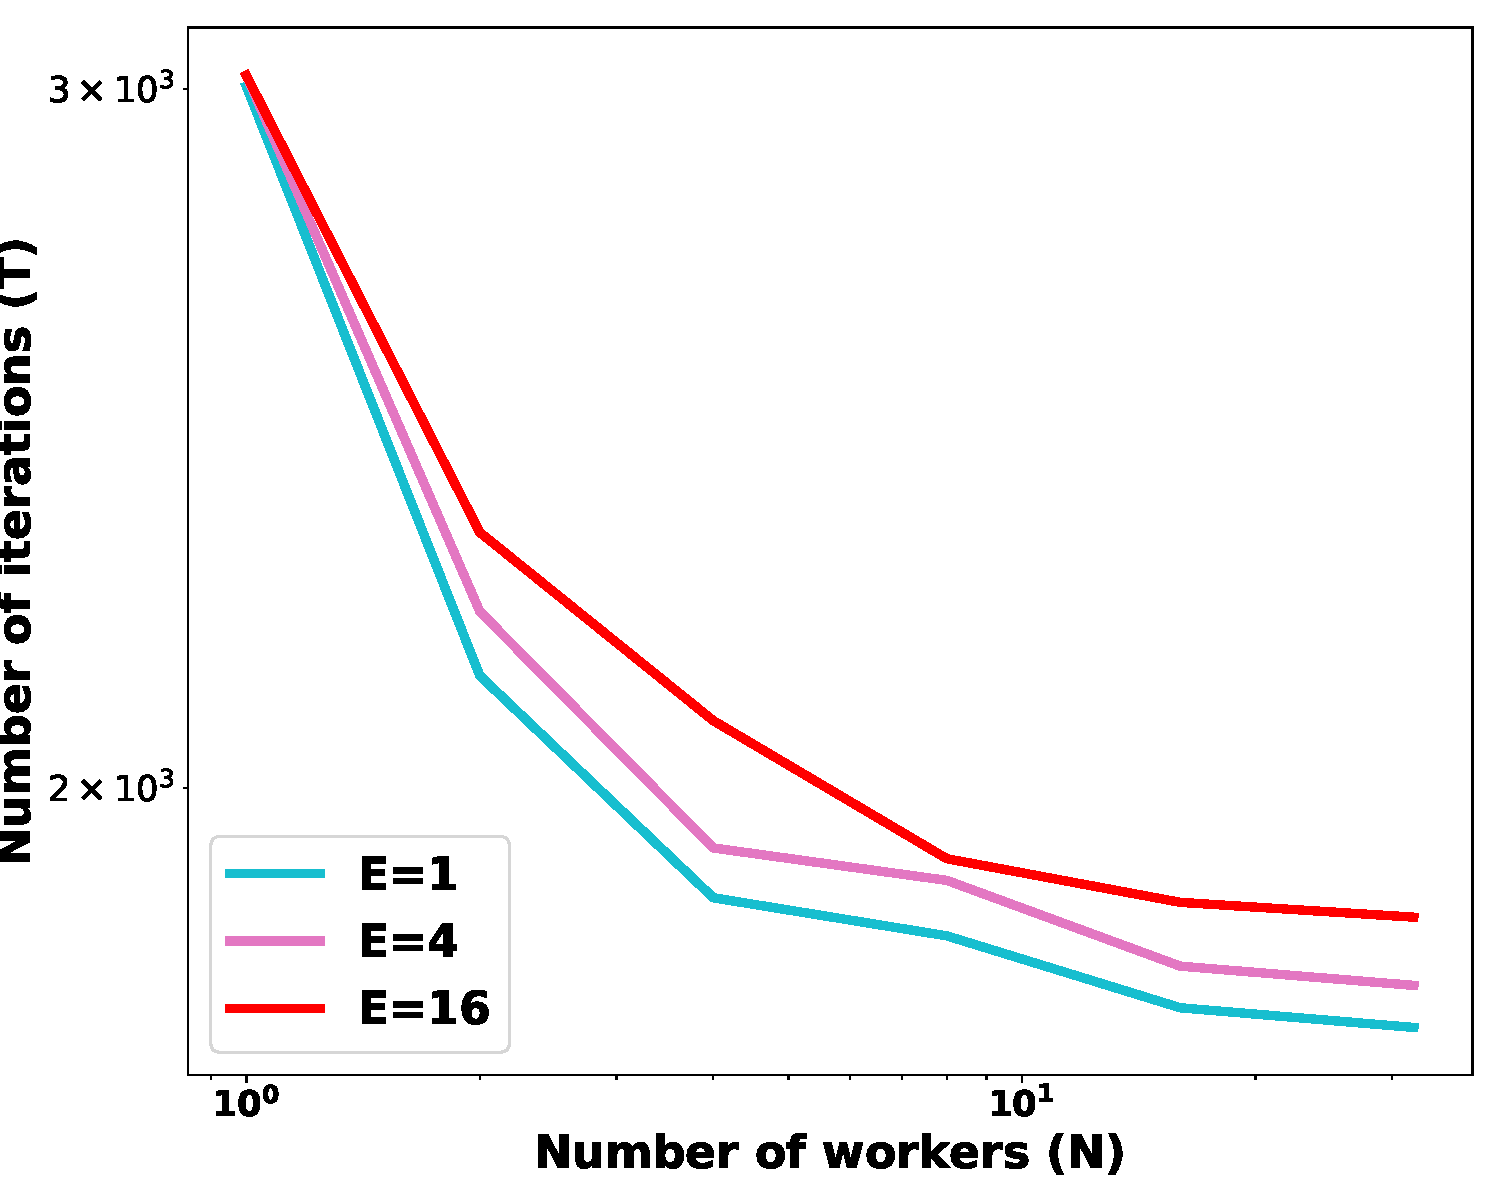
\includegraphics[width=0.33\textwidth]{fig/paper-lrnesterovspeedupNodesT-min-linearregressionw8a-epsilon002-reg0.pdf}\\
(a) Strongly convex objective & (b) Convex smooth objective & (c) Linear regression
	\end{tabular}}
	\vspace{-1em}
\caption{The linear speedup of FedAvg in full participation, partial participation, and the linear speedup of Nesterov accelerated FedAvg, respectively.
% \textbf{Linear speedup } The first row reports the linear speedup convergence of FedAvg w.r.t the number of workers. The second row reports the linear speedup convergence of FedAvg w.r.t the number of active workers in the partial parcipation setting. The third row reports the linear speedup convergence of Nesterov accelerated FedAvg in full participation setting. 
}
\vspace{-1em}
\label{fig:speedup}
\end{figure}

% \begin{figure}
% \centering
% 	\begin{tabular}{ccc}
% 	\hspace{-2em}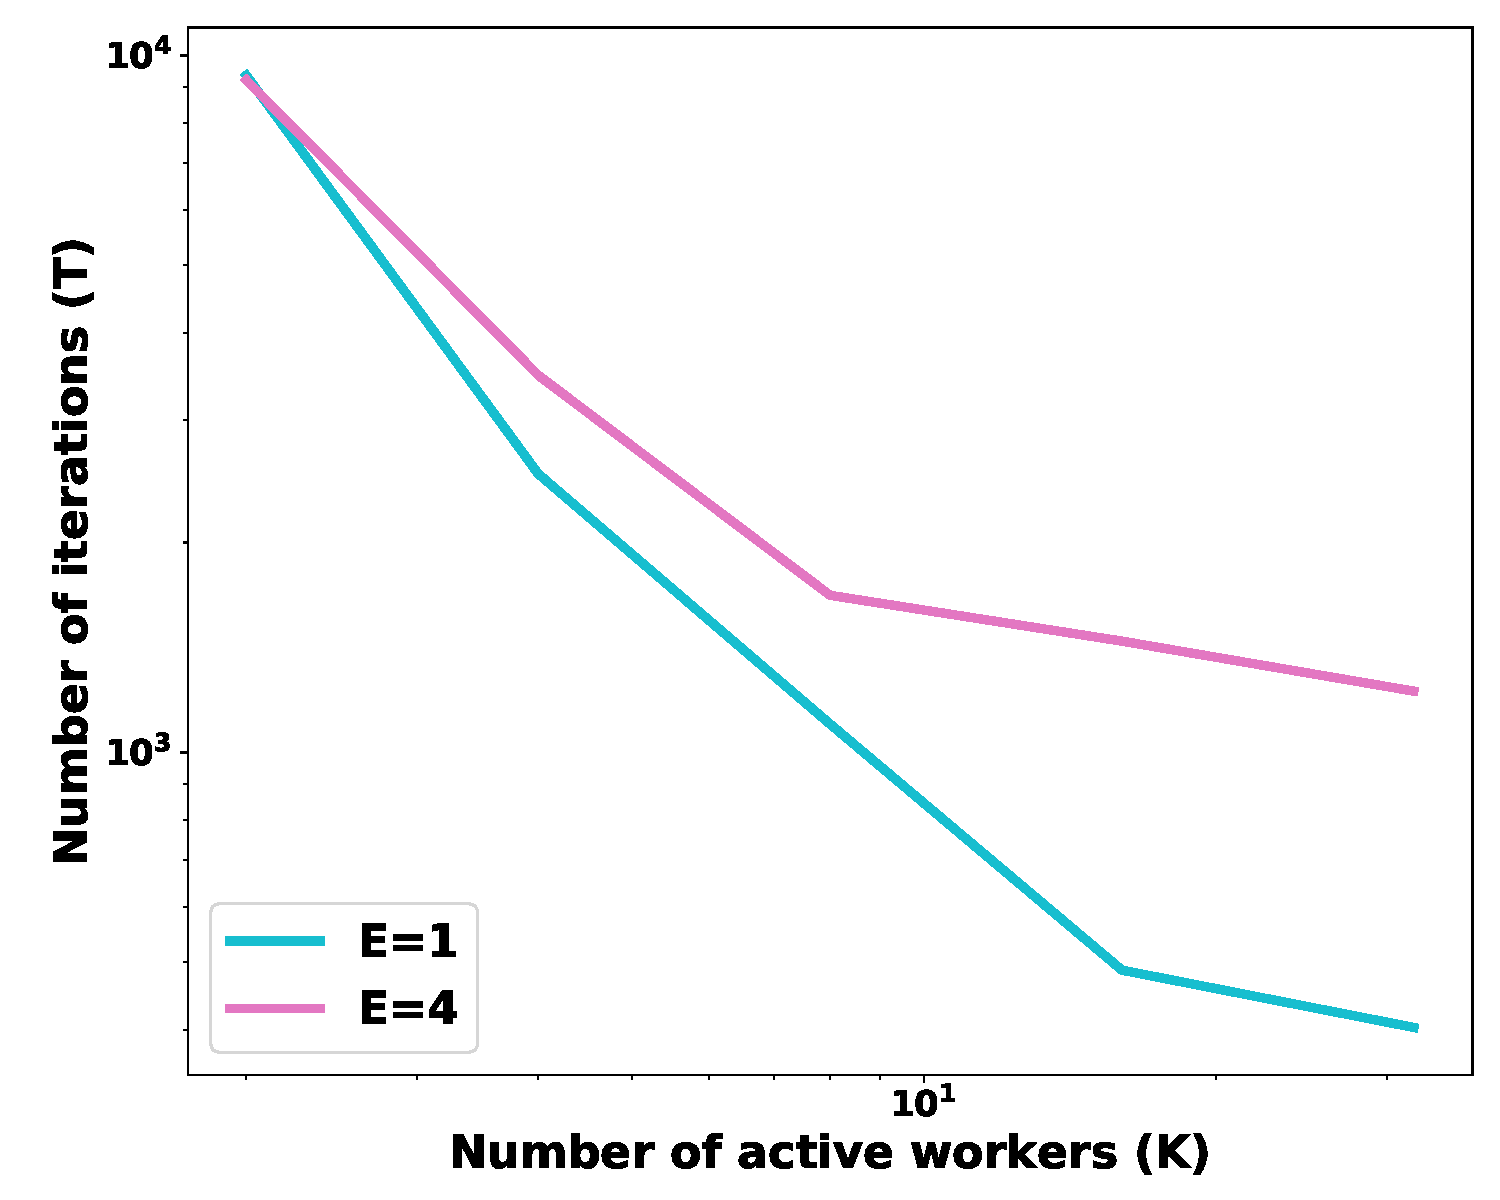
\includegraphics[width=0.33\textwidth]{fig/paper-partialstronglycvxsmthspeedupNodesT-min-w8a-epsilon0131-reg1e-05.pdf} &
% 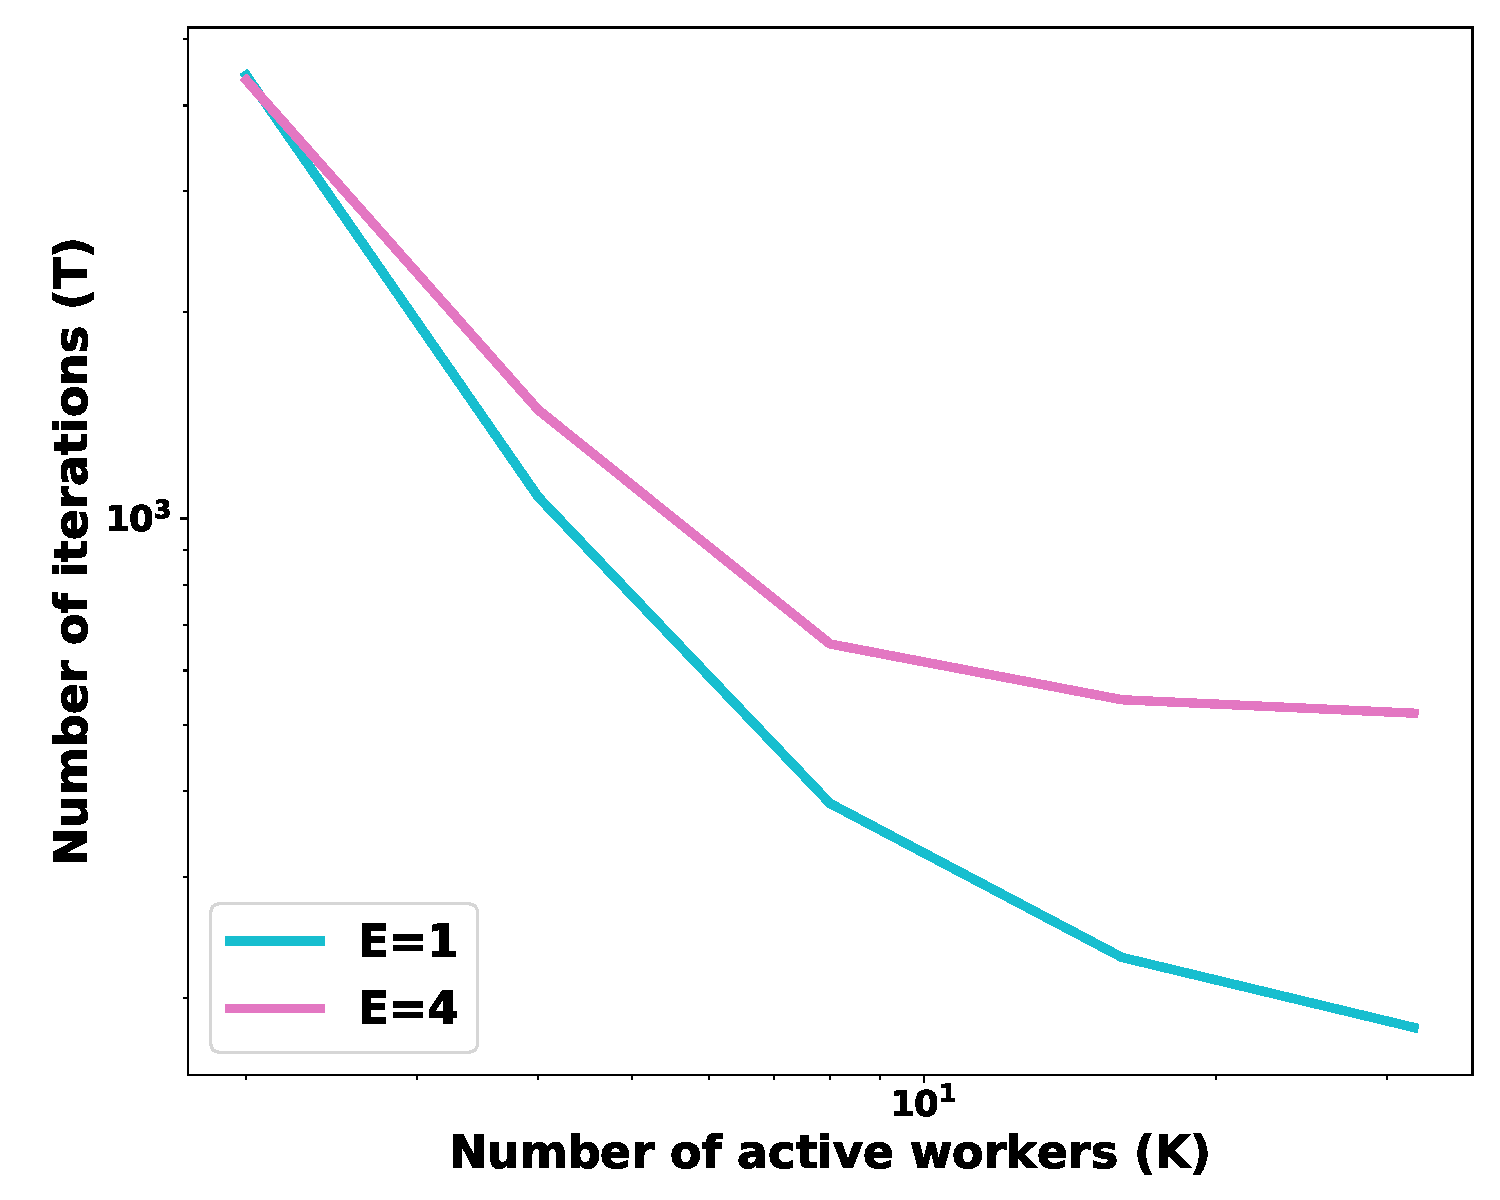
\includegraphics[width=0.33\textwidth]{fig/paper-partialcvxsmoothspeedupNodesT-min-w8a-epsilon0134-reg0.pdf} &
% 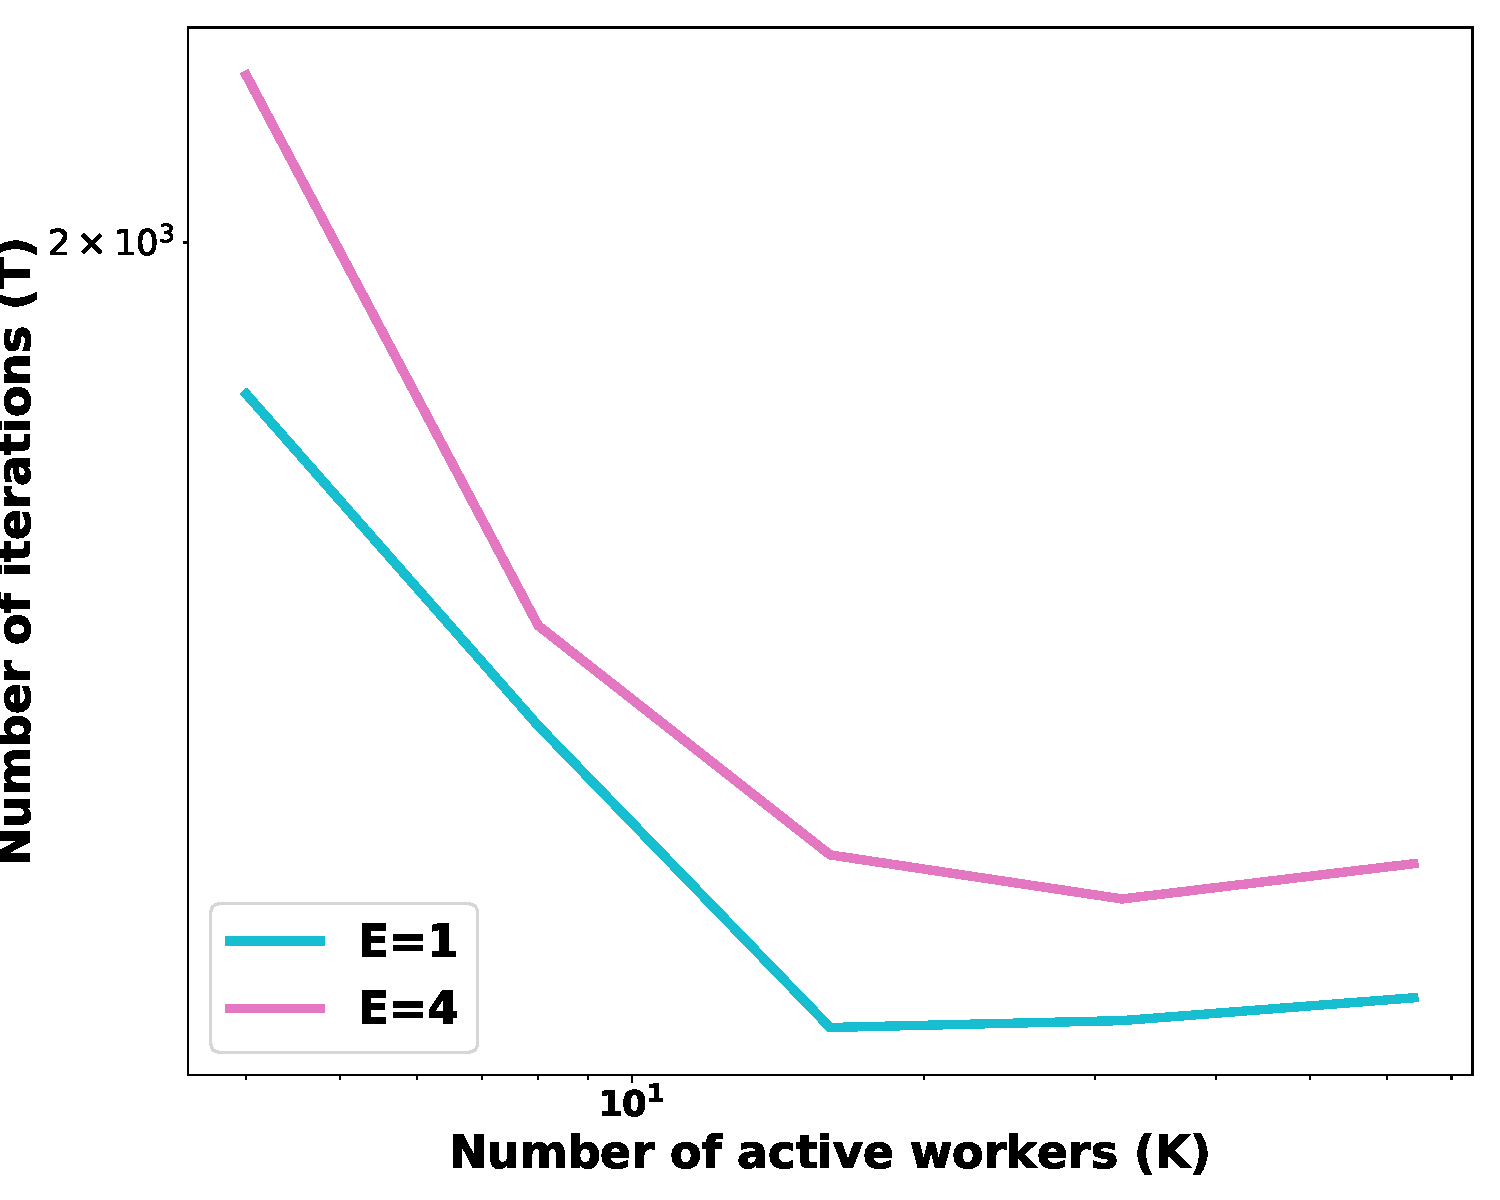
\includegraphics[width=0.33\textwidth]{fig/paper-partiallinregressionspeedupNodesT-min-linearregressionw8a-epsilon002-reg0.pdf}\\
% (a) Strongly convex objective & (b) Convex smooth objective & (c) Linear regression
% 	\end{tabular}
% \caption{The linear speedup convergence of FedAvg w.r.t the number of active workers. }
% \vspace{-2em}
% \label{fig:partial}
% \end{figure}


% \begin{figure}
% \centering
% \begin{tabular}{ccc}
% \hspace{-2em}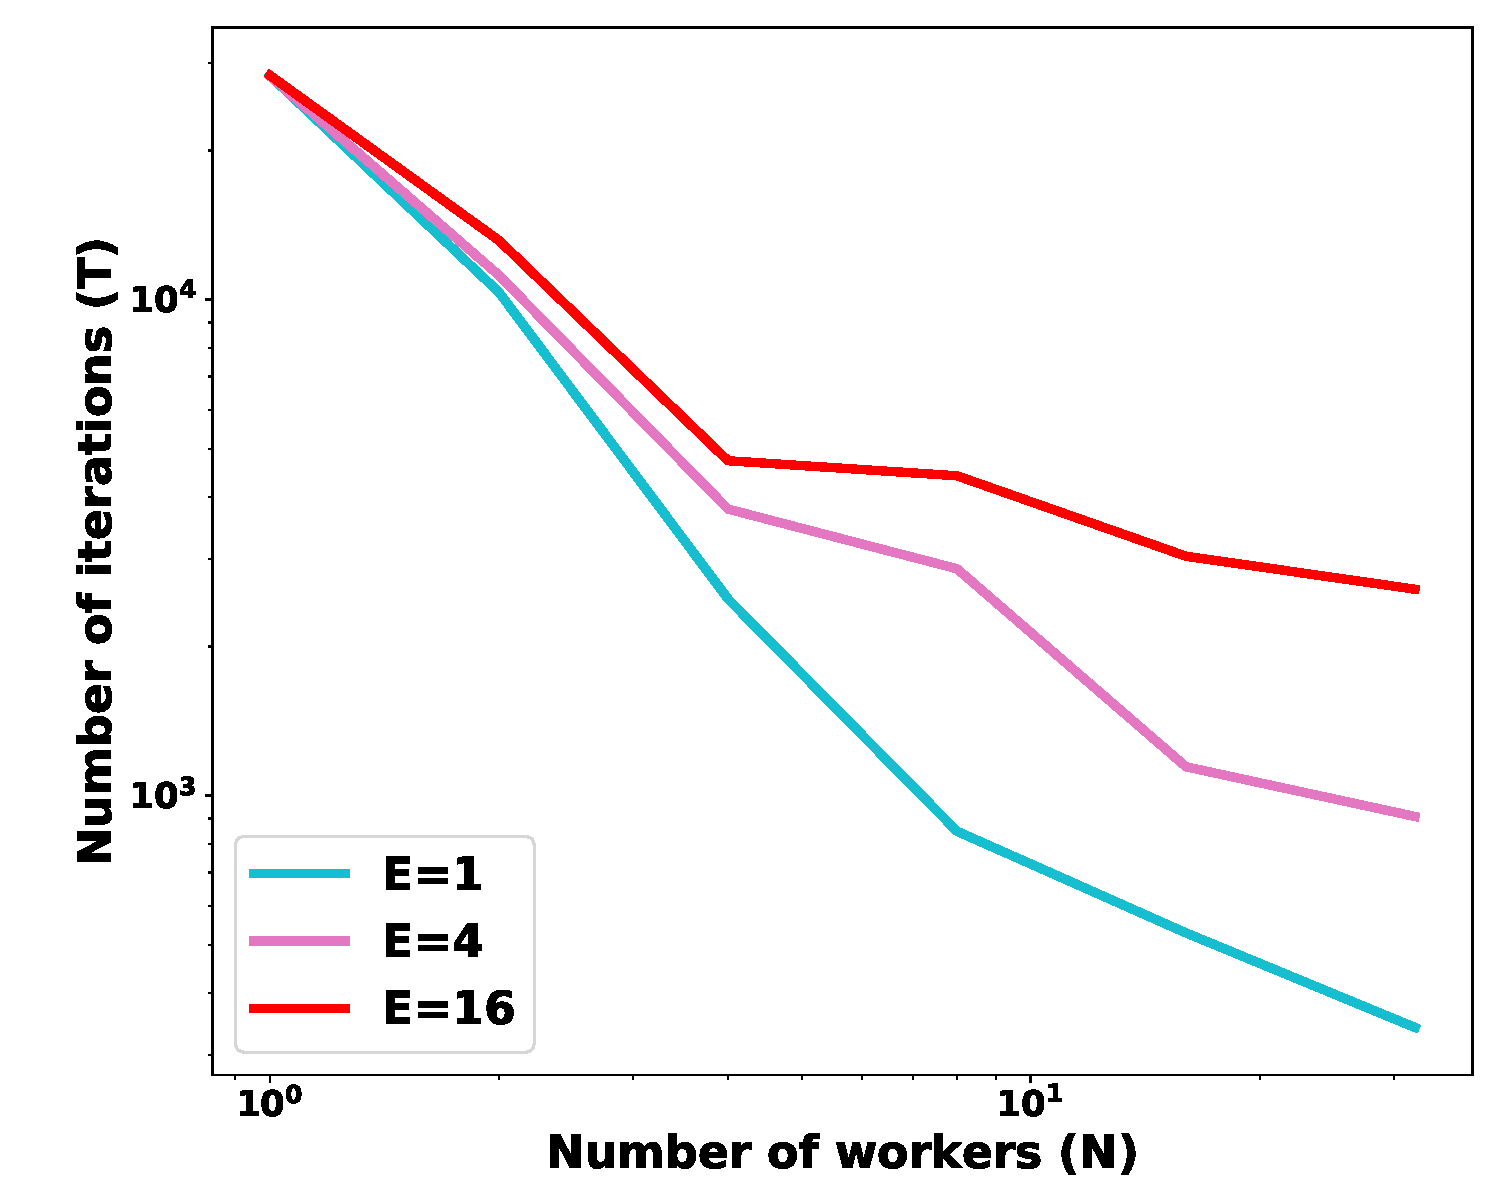
\includegraphics[width=0.33\textwidth]{fig/paper-nesterovspeedupNodesT-min-w8a-epsilon0131-reg1e-05.pdf} & 
% 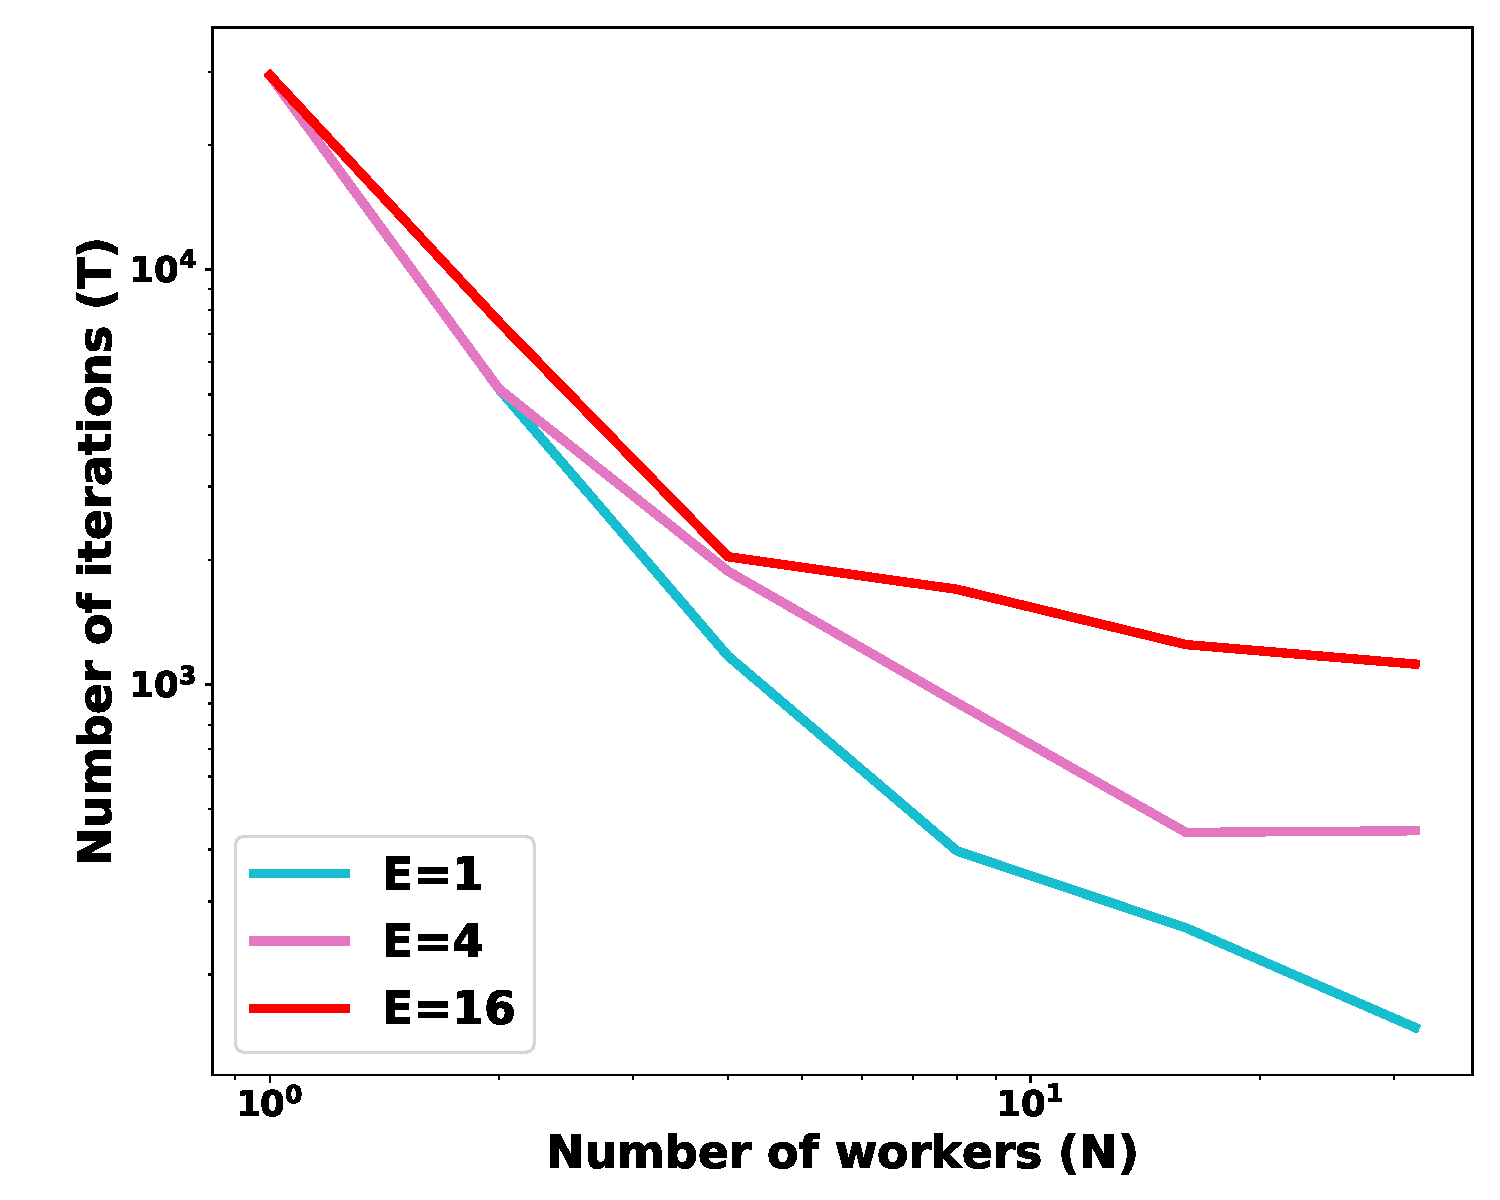
\includegraphics[width=0.33\textwidth]{fig/paper-nesterovspeedupNodesT-min-w8a-epsilon0134-reg0.pdf}
% & 
% 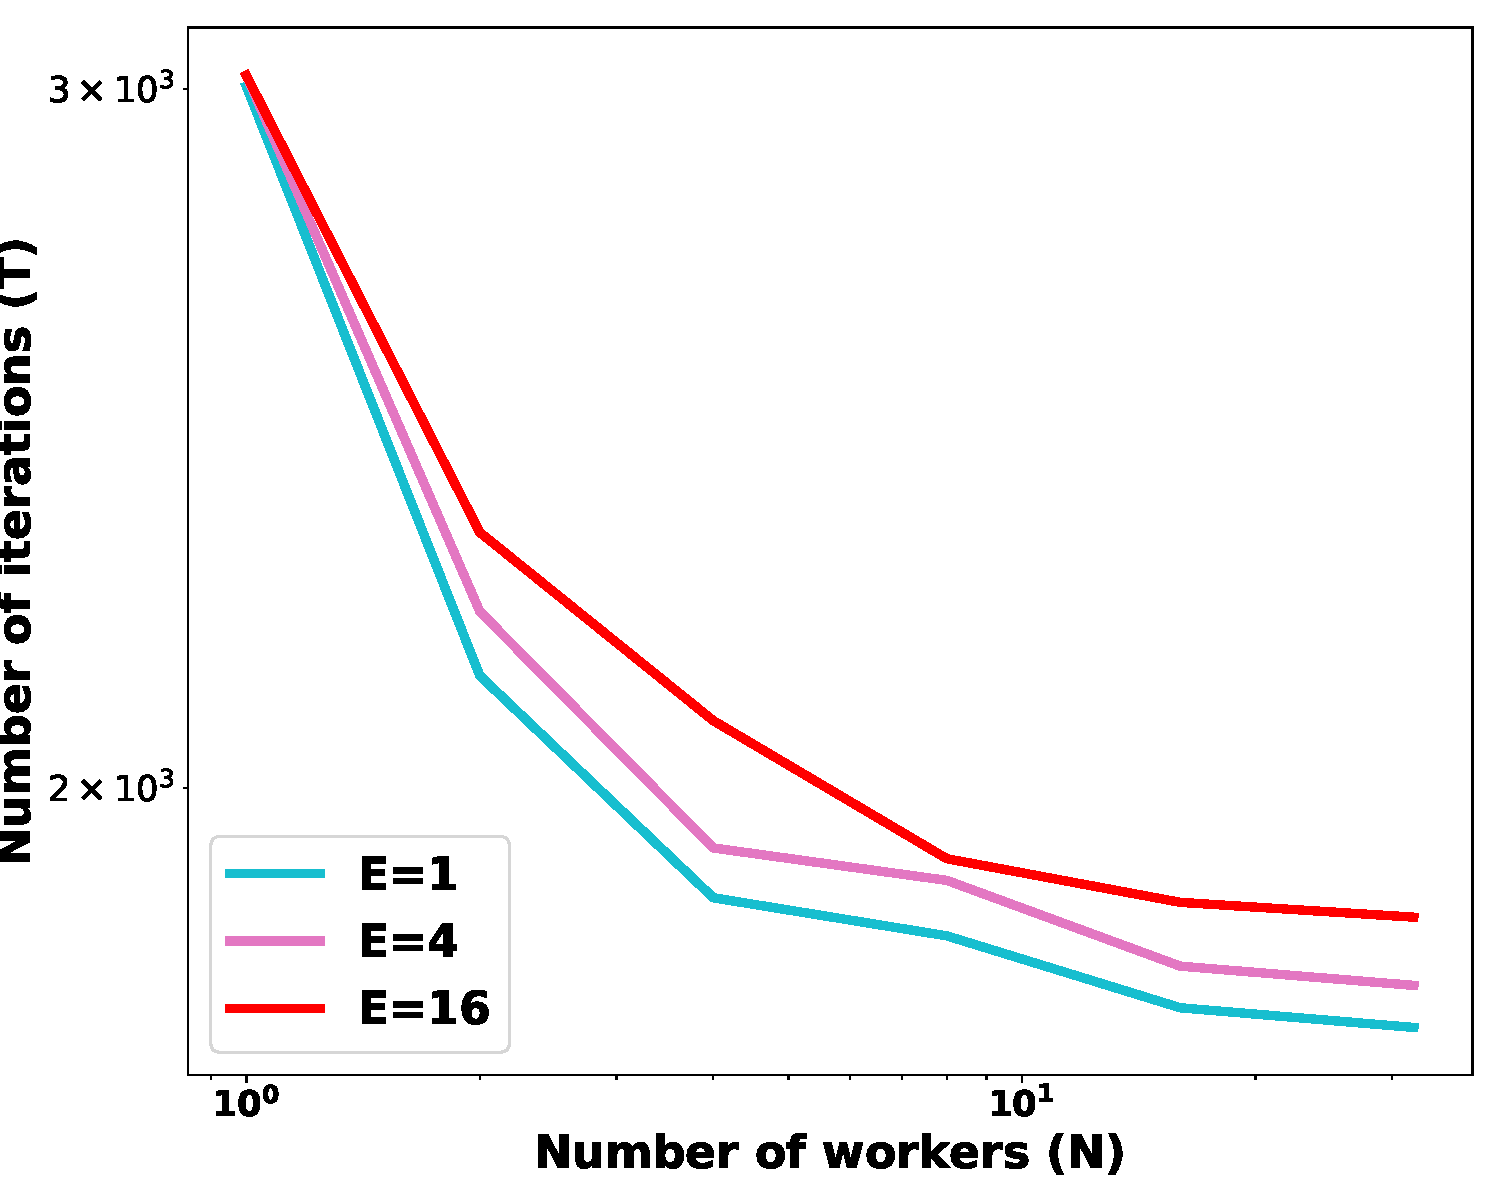
\includegraphics[width=0.33\textwidth]{fig/paper-lrnesterovspeedupNodesT-min-linearregressionw8a-epsilon002-reg0.pdf}\\
% (a) Strongly convex objective & (b) Convex smooth objective & (c) Linear regression
% 	\end{tabular}
% \caption{The linear speedup convergence of Nesterov accelerated FedAvg w.r.t the number of workers. }
% \label{fig:nesterov}
% \end{figure}



% \begin{figure}
% \centering
% 	\begin{tabular}{ccc}
% 	\hspace{-2em} 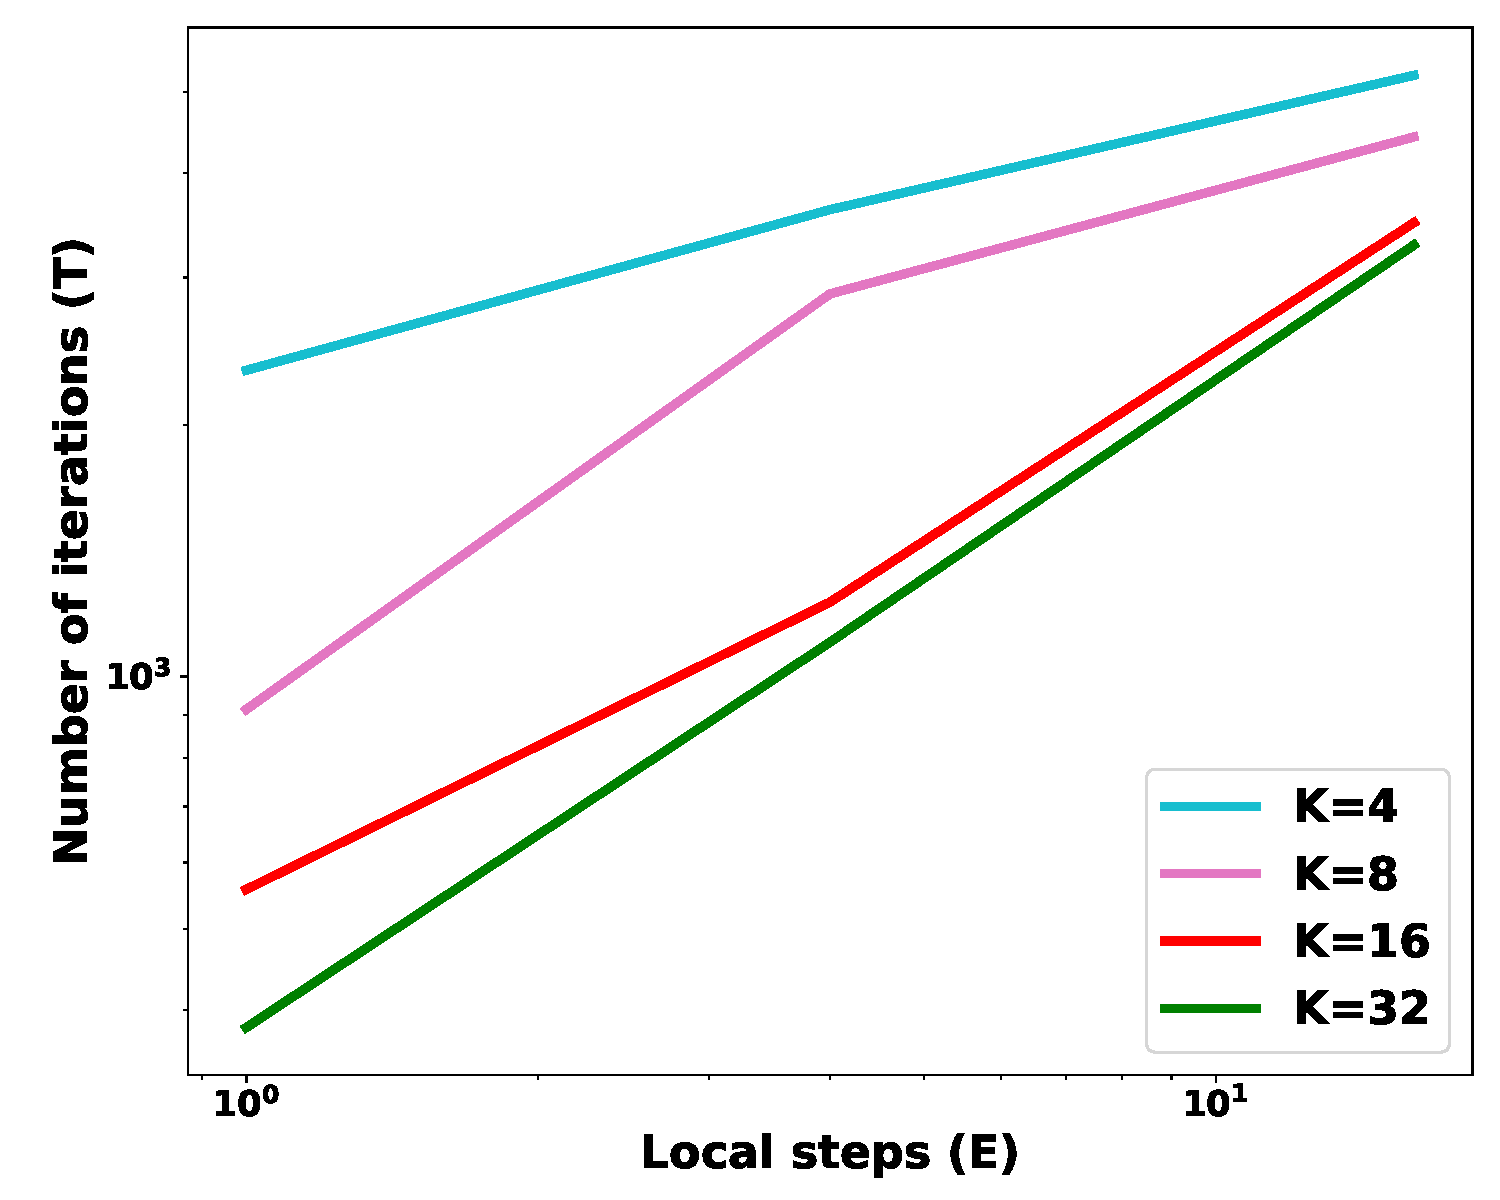
\includegraphics[width=0.33\textwidth]{fig/paper-stronglycvxsmthspeedupEpochsT-min-w8a-epsilon0131-reg1e-05.pdf} &
% 	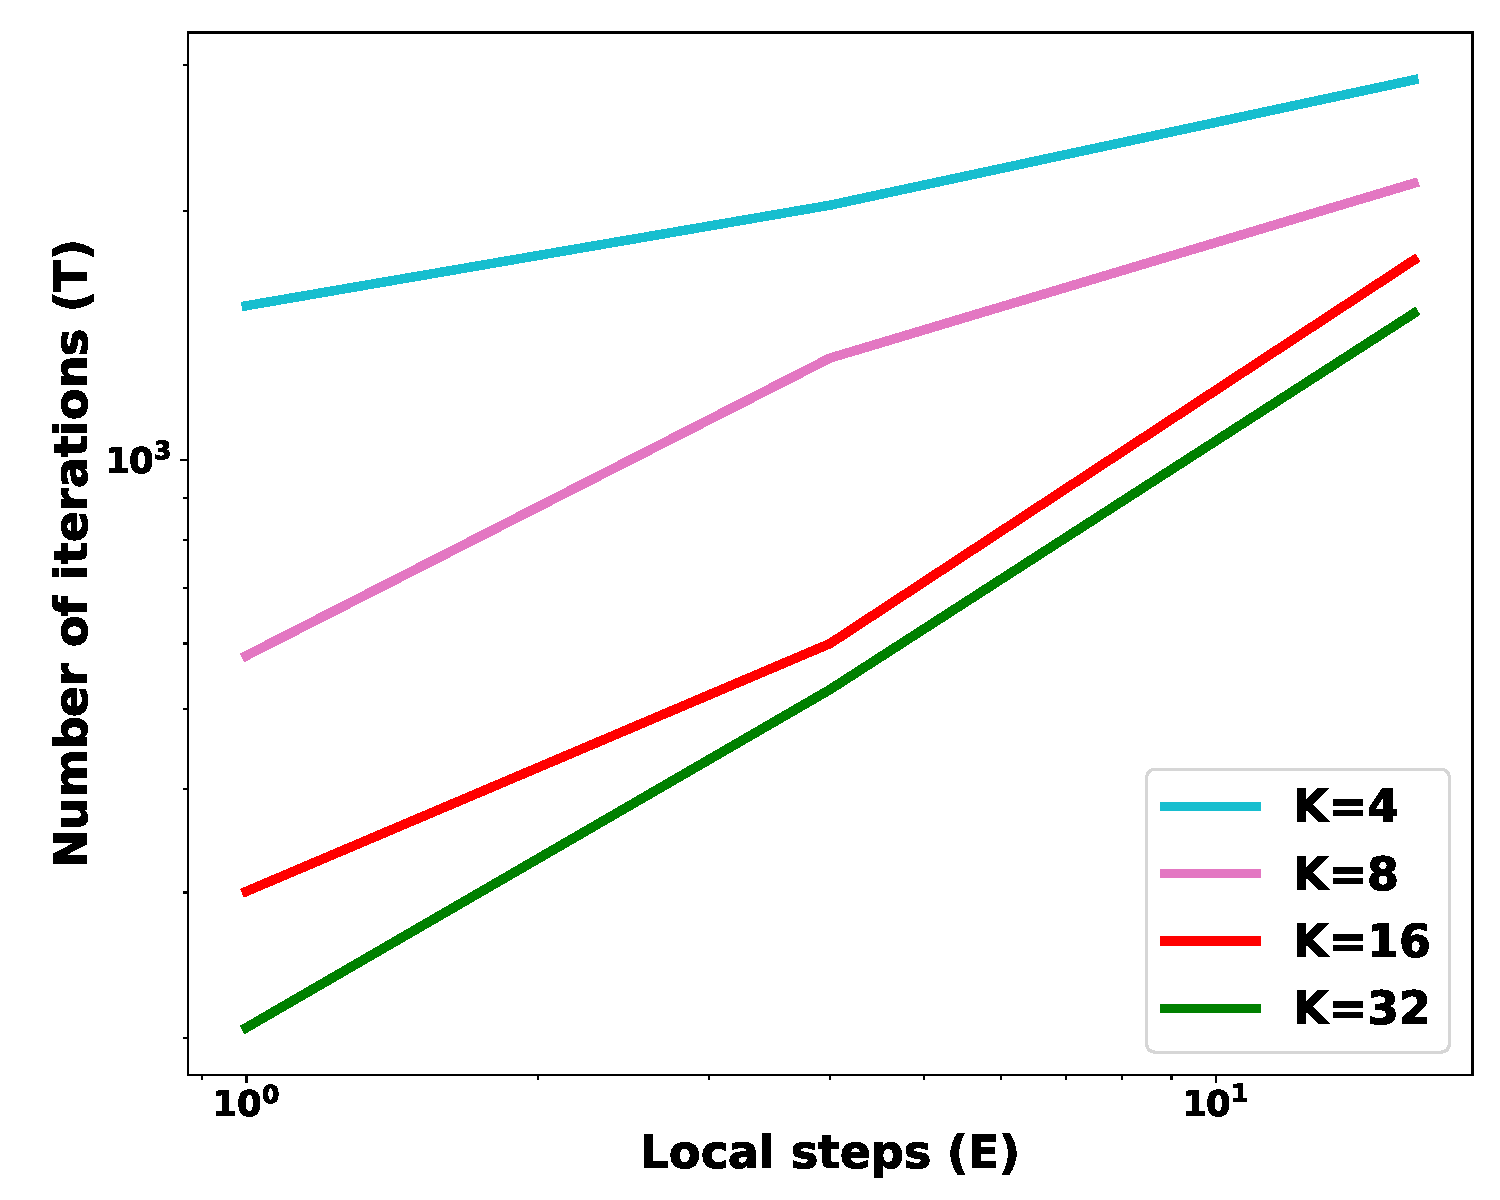
\includegraphics[width=0.33\textwidth]{fig/paper-cvxsmoothspeedupEpochsT-min-w8a-epsilon0134-reg0.pdf} & 
% 	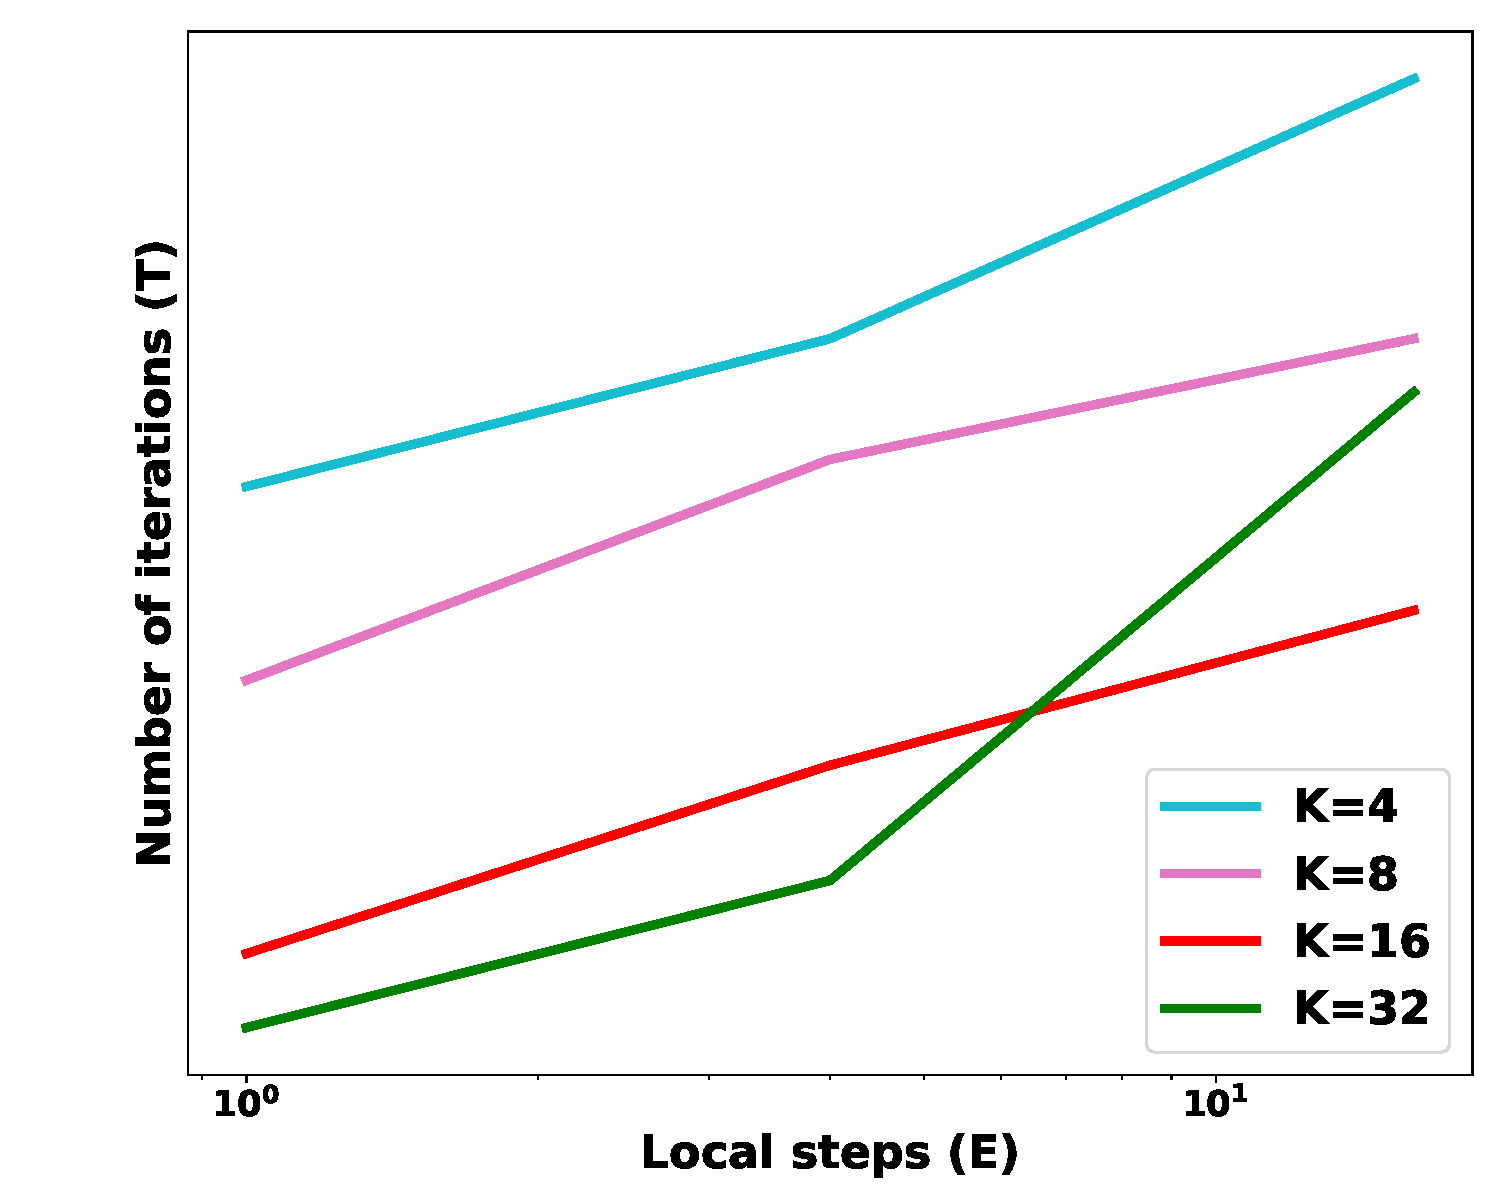
\includegraphics[width=0.33\textwidth]{fig/paper-linregression-newspeedupEpochsT-min-linearregressionw8a-epsilon002-reg0.pdf} \\
% 	\hspace{-2em} 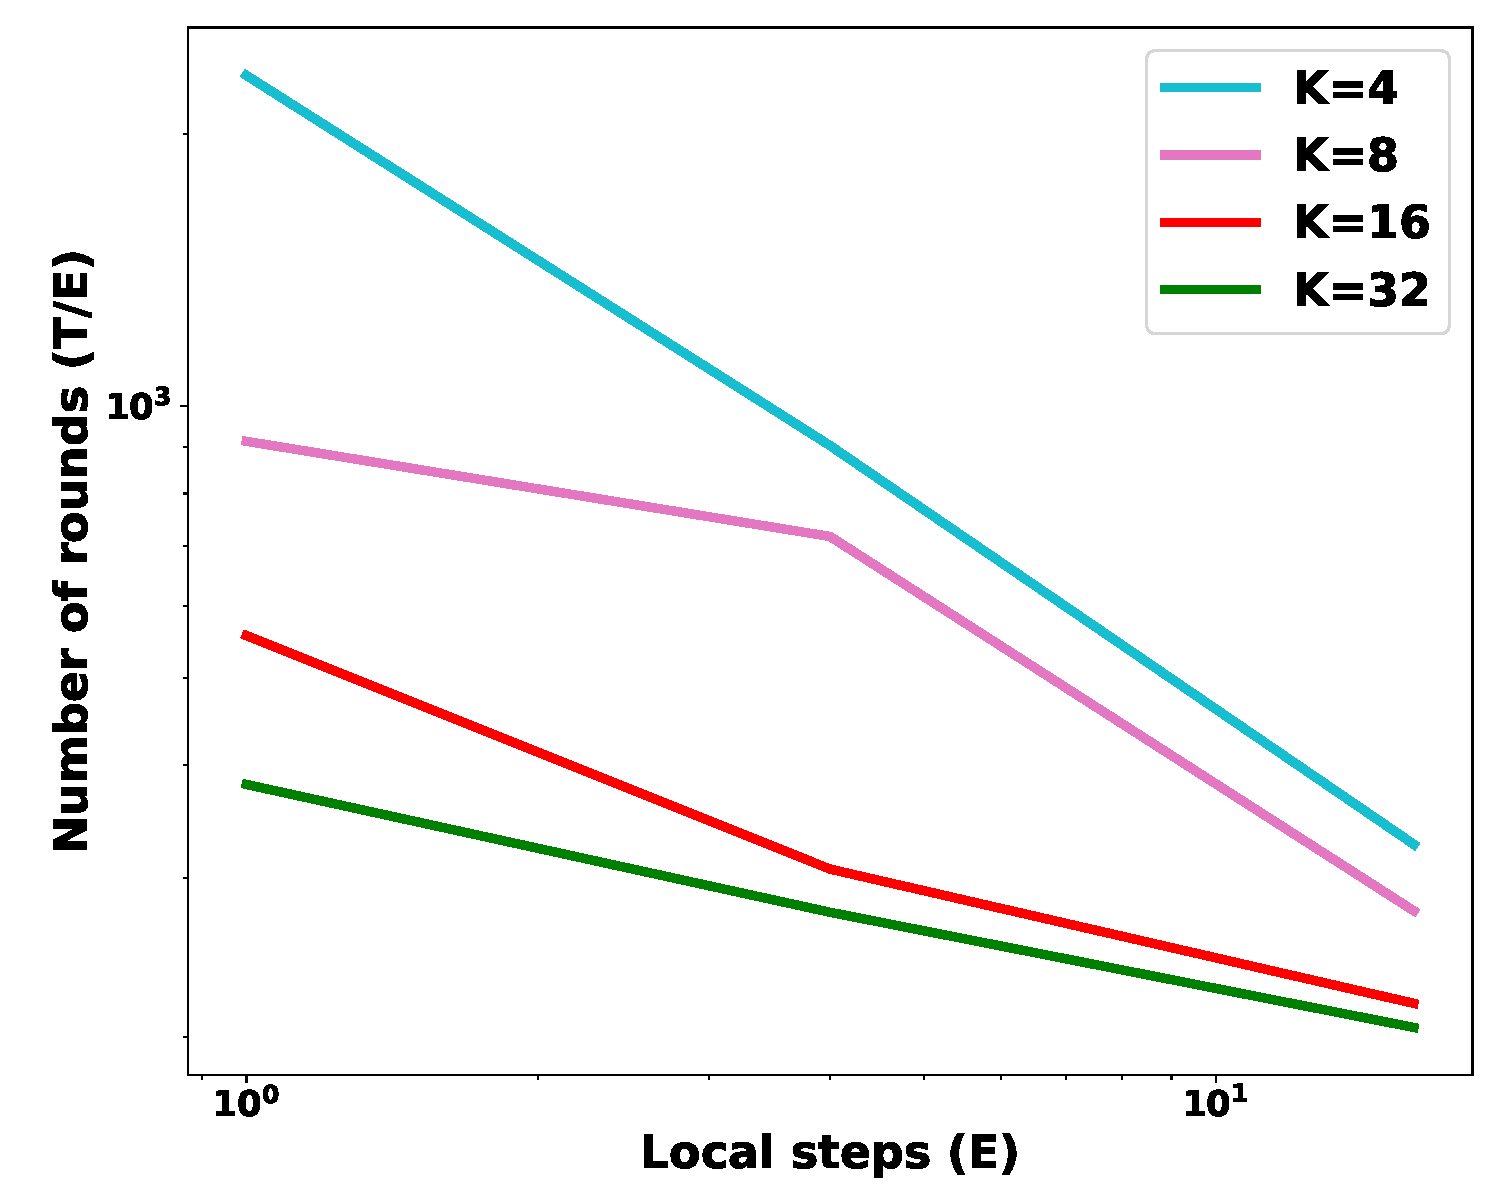
\includegraphics[width=0.33\textwidth]{fig/paper-stronglycvxsmthspeedupEpochsRounds-min-w8a-epsilon0131-reg1e-05.pdf} &
% 	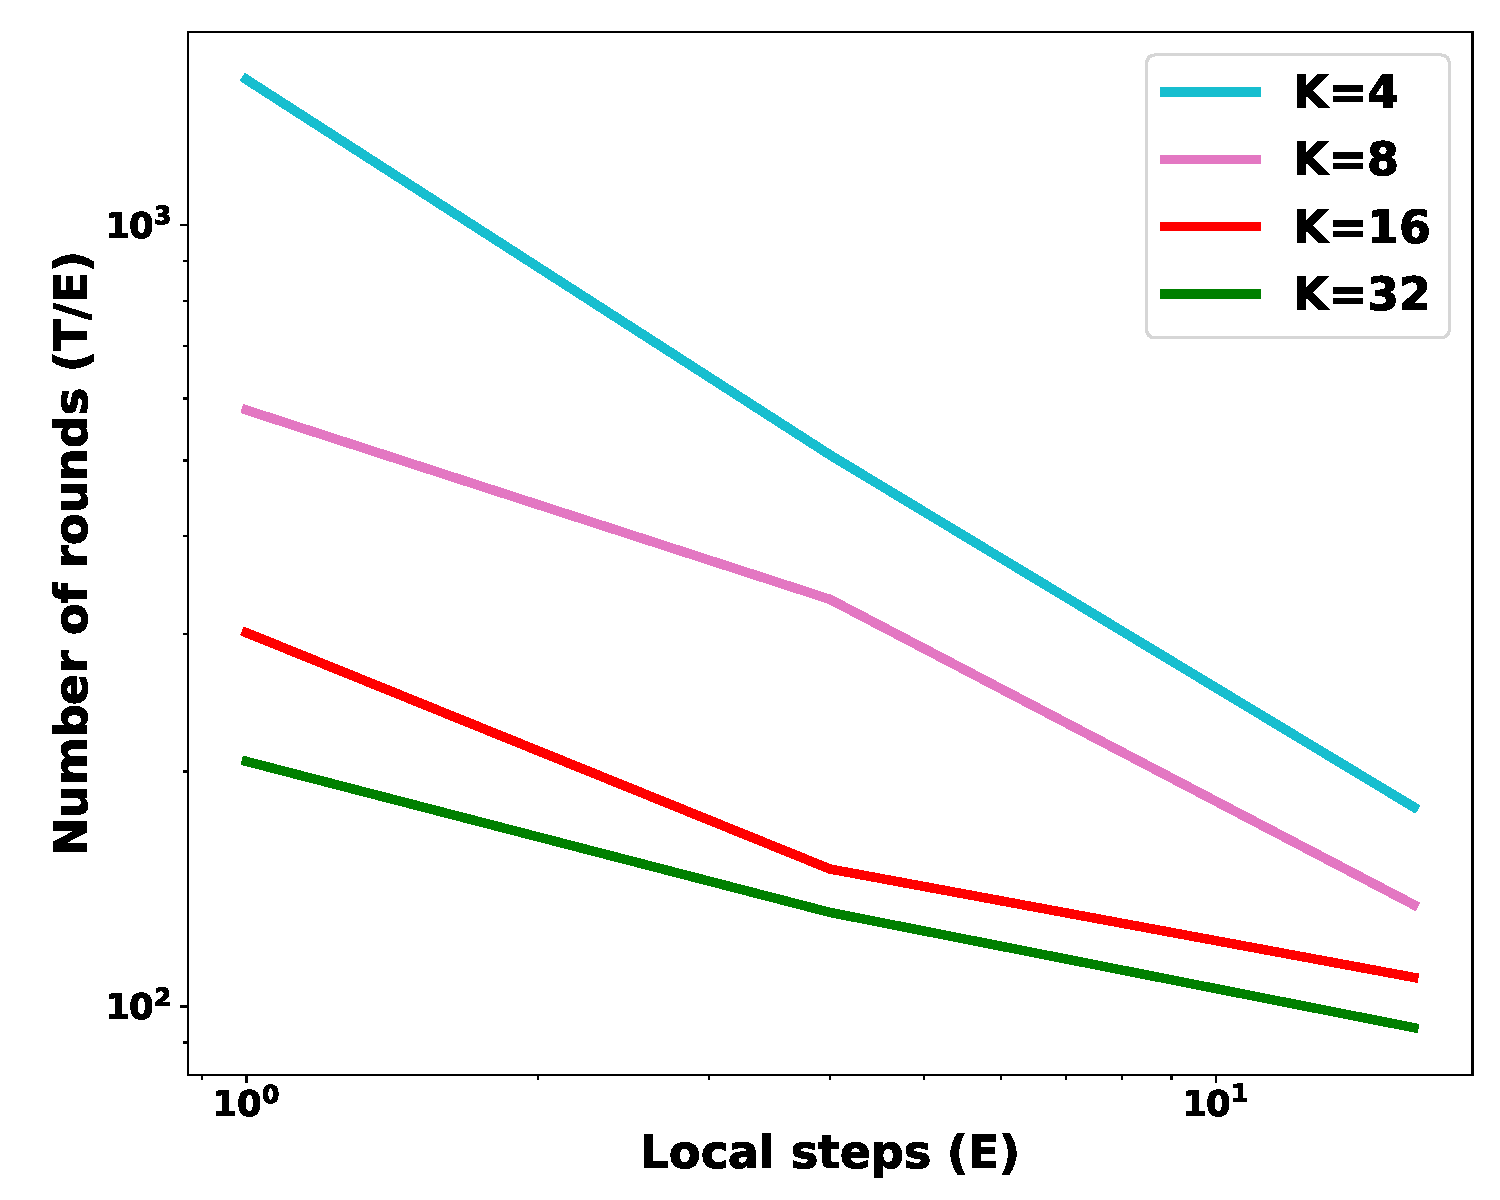
\includegraphics[width=0.33\textwidth]{fig/paper-cvxsmoothspeedupEpochsRounds-min-w8a-epsilon0134-reg0.pdf} & 
% 	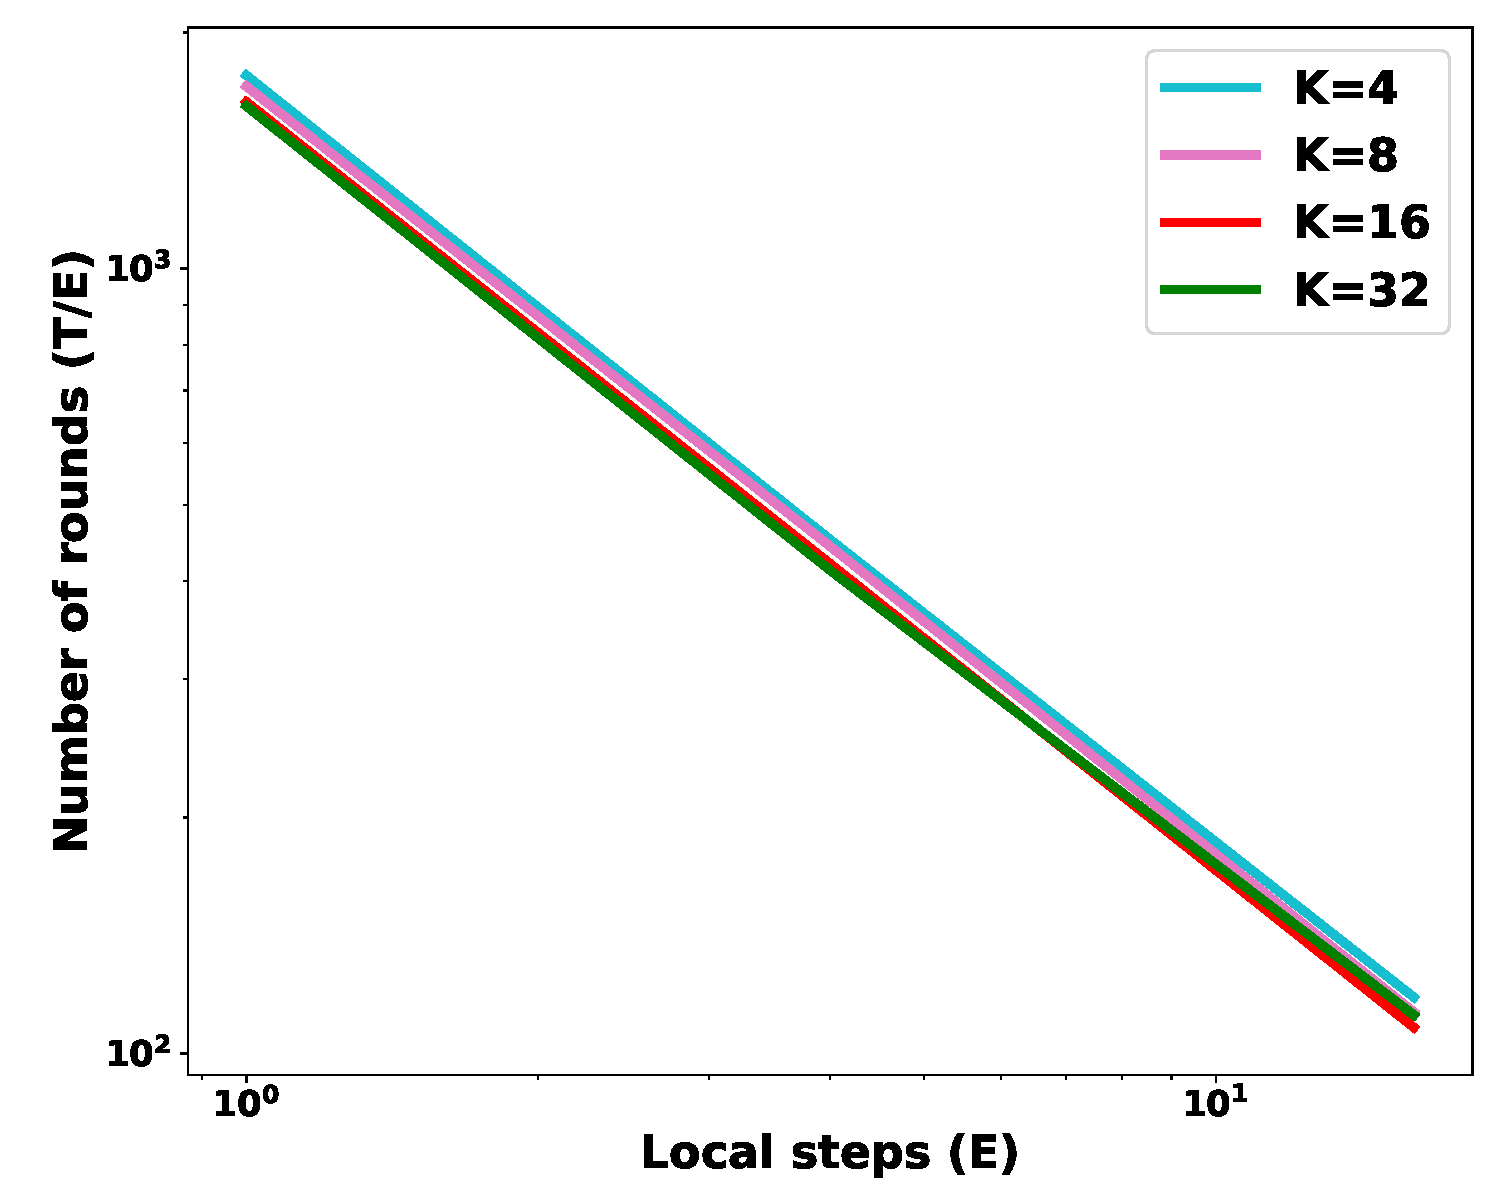
\includegraphics[width=0.33\textwidth]{fig/paper-linregression-newspeedupEpochsRounds-min-linearregressionw8a-epsilon002-reg0.pdf} \\
% (a) Strongly convex objective & (b) Convex smooth objective & (c) Linear regression
% 	\end{tabular}
% \caption{The convergence of FedAvg w.r.t the number of local steps $E$. }
% \label{fig:e}
% \end{figure}



